% don't remove the following lines, and edit the definition of \main if needed
%\documentclass[../report.tex]{subfiles}
%\providecommand{\main}{..}
%\usepackage[normalem]{ulem}
%%\usepackage{colour}
%\IfEq{\jobname}{\currfilebase}{\AtEndDocument{\biblio}}{}
% until here

%To have the comments written on the PDF: keep this macro
%\newcommand{\commentsinout}[1]{#1}
%To have the comments hidden in the PDF: keep this macro
%\newcommand{\commentsinout}[1]{}

% this is a macro so you can make comments. See example below.
%\newcommand{\JDH}[1]{\commentsinout{{\bf{\color{brown} [JDH: #1]}}}} % Comments by Jorgen D'Hondt
%\newcommand{\KR}[1]{\commentsinout{{\bf{\color{cyan} [KR: #1]}}}} % Comments by Krzysztof Redlich

%\usepackage{lineno}

%\renewcommand{\sout}{\bgroup\color{blue} \ULdepth=-.5ex \ULset}

%%\linenumbers

\begin{document}
\linenumbers
\chapter{Strong Interactions}
\label{chap:si}
%\corr{Introduction to the chapter or the next subsection is already a quite good intro? }
%We defined some small macros to allow comments to be made. For instance \JDH{this is a comment by Jorgen}. Reference~\cite{Mangano:2270978}. They are to be added in bibtex format under the directory section1 and bib in the file section.bib.

%\JDH{Intention is to stick to 10 pages total. The count below, including some figures reaches about 14 pages which was discussed in the PPG and this length is still fine.}

%%%%%%%%%%%%%%%%%%%%%%%%%%%%%%%%%%%%%%%%%%%%%%%%%%%%%%%%%%%%%%%%%%%%%%%%%%%%%%%%%

%\JDH{1.5p}} \JDH{editor: Jorgen}\\

%General introduction of \JDH{0.5p}
%\begin{itemize}
%\item Introduction to QCD from theory to phenomena, in both the high-$\alpha_s$ and %low-$\alpha_s$ regime, i.e. the confined and vacuum regime. Comprehensive introduction to %the level to appreciate the key objectives as defined in the following subsections.
%\item Our understanding of $\alpha_s(Q^2)$ on the experimental side and the theoretical %side.
%\end{itemize}https://www.overleaf.com/project/5ce2fdf82fe231531842b32a

%\JDH{Merged the text of Thomas and Uta, see below}

%From Thomas
\section{State-of-the-art}
Quantum Chromodynamics (QCD) is firmly established as the theory of strong interactions. The dynamics of quarks and gluons is encoded in %\sout{a remarkably simple} 
a locally SU(3) invariant Lagrangian density, which predicts and explains a plethora of experimentally observed phenomena. The dependence of the QCD coupling $\alpha_s(Q)$ on the energy scale $Q$ is predicted in QCD to evolve from a strong coupling at low scales to a weak coupling at high scales. As a consequence, quarks and gluons are confined into hadronic bound states at low energies, while behaving asymptotically free at high energies. 

The concept of asymptotic freedom enables precise quantitative predictions for QCD processes at high energy colliders, obtained in a systematic manner using perturbation theory. To allow the full exploitation of precision collider data, these calculations need to attain high accuracy and precision, which goes along with conceptual and technical challenges in perturbative calculations and event simulation. Alterations of QCD may still become manifest, such as the embedding of QCD in a higher gauge theory possibly unifying electroweak and strong interactions, the discovery of unbound colour or of a new level of substructure. At low scales and/or high density, the quantitative understanding of QCD is less fully developed, with the first-principles understanding of confinement as an outstanding open question. The  evaluation of  nonperturbative contributions arising
in QCD  is however   possible     within numerical lattice QCD (LQCD). Furthermore,  synergies of QCD with adjacent fields are identified, e.g., with string theory through the use of the Ads/CFT correspondence for a strongly coupled gauge theory,
% the use of the AdS/CFT correspondence for a strongly coupled gauge theory in string theory
and the strong CP problem potentially related to axion-like cold dark matter and the neutron EDM.

The separation of low-energy and high-energy dynamics through QCD factorisation is a cornerstone of particle physics phenomenology, enabling precision predictions for collider processes by parametrising the strong-coupling dynamics into empirical quantities such as decay form factors, parton distributions or hadronisation models. These have often dual relevance, as fundamental objects of investigation and as input to predictions, depending on the research question under consideration. Future progress in fundamental understanding and precision phenomenology of QCD will rely on a diverse research programme with close interplay between theoretical advances and experimental measurements. 
\vfill
%From Uta

%QCD is the gauge field theory of strong interactions which emerged after the discovery of quarks, in ep, and later with the discovery of gluons, in $\Pep\Pem. It has been very successfully tested and applied in the interpretation of high energy measurements and led to a radically new understanding of strong interactions and substructure. Major alterations of QCD may still become manifest~\cite{Quigg:2013lya}, such as the embedding of QCD in a higher gauge theory possibly unifying electroweak and strong interactions, the discovery of unbound colour or of a new level of substructure. 
%The confinement question, called one of the millennium puzzles~\cite{Jaffe:2000ne}, remains to be explained still. Possible relations of QCD to string theory and the use of gravitation techniques (AdS/CFT) to develop theory further deserve to be explored as well as the CP violation related to axions, which may explain dark matter. 
%Principal questions in QCD such as the existence of instantons, the phenomenon of diffraction in high-energy collisions, new dynamics at high parton densities and the onset of long-range particle correlations are just examples that ought to be studied much deeper. A qualitatively and quantitatively new level is required in the understanding of parton dynamics encoded in the structure of the proton and QCD theory to maximise the physics outcome of the LHC QCD, electroweak, Higgs and BSM programme, and the reliable preparation of a future higher energy hadron collider.

%Proton structure extends to three dimensions, and a new field of research, related to generalised and unintegrated parton distributions, is to be explored. Huge deficits exist in the understanding of the partonic structure of the neutron, deuteron, pion, photon, Pomeron and nuclei. The relation of QCD as a gauge field theory to collective phenomena studied in heavy and lighter ion collisions is far from being understood. Parton structure and dynamics in nuclei lacks experimental input as it relies on fixed target muon-hadron experiments mainly. Nuclear substructure is completely unresolved at small $x$, and has to be probed at scales set by the LHC and higher energy colliders.

%QCD is complex and fundamental, it has to be developed further through new experiments, for which eA and ee colliders have special roles in probing the nucleon structure and the mechanism of hadronisation. QCD is of fundamental importance, which may be further illustrated with the unsatisfactory status of the determination of $\alpha_s$, the least known fundamental coupling constant, or with the relevance that the measurements of PDFs at small $x$ have for neutrino astrophysics.



%\JDH{0.5p, plus a figure}}
\label{section_low}
%\begin{itemize}
%\item Key overall objectives.
%\item Experimental knowledge about PDFs and theoretical progress. Impact on the LHC physics programme.
%\item Main challenges, experimental and theoretical.
%\end{itemize}

%\JDH{quantify the impact of current and future PDF fits on Higgs cross sections?}
\subsection{The low-$\alpha_s$ or vacuum regime}
The partonic structure of hadrons is described in terms of Parton Distribution
Functions (PDFs) where QCD provides with the DGLAP equations only a prediction of the evolution of their structure with the energy scale. Especially the experiments at the HERA facility at DESY provided Deep Inelastic electron- and positron-proton Scattering (DIS) data to determine the PDFs covering a significant part of the $Q^2$ versus $x$ plane.
%
The use of these PDFs in certain kinematic ranges probed in pp collisions at the
LHC (and even more at the FCC or CEPC-pp) propagates into large systematic uncertainties
for key theoretical predictions.
%The extrapolation of these PDFs to predictions in the kinematic range probed with the LHC induces large systematic uncertainties.
Proposals are submitted to address this by extending the kinematic domain with new collider and fixed-target experiments.
%
%Electroweak and Higgs physics at the LHC enter the precision era demanding a new level of understanding QCD, especially of the proton structure and of $\alpha_s$.

Electroweak and Higgs physics at the LHC are entering the precision era, demanding a new level of understanding QCD, including questions related to proton structure and, the value of the strong coupling ($\alpha_s$), calculation of higher order matrix elements, the understanding of multi-scale problems through parton showers and resummations, and effects related to hadronisation.
Measurements performed at the HL-LHC of important EW parameters like the W boson mass~\cite{ATL-Wmass} and $\sin^2\theta_W$~\cite{ATL} can be significantly improved when more profound (from PDFs to GDPs) and extended (to higher $Q^2$, and both higher and lower $x$) information becomes available on the proton structure.
% show impressively the gain of ep and pp collider physics, where e.g. the PDF uncertainty of sin2theta is expected to be reduced by an additional factor of 5 with respect to the one obtained with the HL-LHC prospect PDFs.
Similarly, the full exploitation of the $gg \to H$ cross section at N$^3$LO (see Sec. \ref{precision_sec}) envisaged at the HL-LHC requires a consistent N$^3$LO set of PDFs which could be obtained from studies at future ep colliders~\cite{Bruening:2013bga}.
%a prediction of the total Higgs production cross section in $pp$ to within a few per mille accuracy~\cite{Bruening:2013bga}. 
This underlines the importance of measuring the strong coupling at the $Z$ mass, $\alpha_s(m_\text{Z})$,
% measuring $\alpha_s$
to 1--2 per mille precision which is considered to be possible at future $ep$ and $e^+e^-$ colliders~\cite{dEnterria:2019its} and challenges LQCD to reach equivalent precision. 
In the search for new physics, the HL-LHC will explore the largest possible masses  requiring a new understanding of partons, gluon, sea and valence quarks at large $x$ in the proton. Estimates illustrate that large $x$ PDFs obtained at the future LHeC would extend the search range for example for new heavier vector bosons in contact interactions at the HL-LHC by 10~TeV. In order to undoubtedly enable such discoveries the proton structure information has to be obtained independently of constraints derived from the $pp$ collisions themselves. 
%Beyond PDF constraints obtained from $pp$ it will be thus crucial to obtain new input from high energy ep colliders, especially the LHeC. 
Very precise PDFs obtained in $ep$ collisions would establish as well a new base for testing QCD factorisation and evolving QCD theory by isolating novel dynamics. 
%It has been estimated that knowing the large $x$ PDFs would enable pp to use its full statistical power to extend the search range for example for new heavier vector bosons in contact interactions by 10 TeV without current PDF systematic limitations.  
HL-LHC detectors upgrades will enable the explorations into the forward region probing the low Bjorken-$x$ range. Future $ep$,  $eA$  and $pp$ colliders like the LHeC,  FCC-ep, es well as  FCC-pp and  CEPC-pp  have the potential to %uniquely 
answer the question of where 
non-linear parton (especially gluon) evolution sets in. These would fundamentally change the pattern of parton evolution and enhance the numerical predictions of cross sections envisaged at high-energy FCC-hh 
%hadron colliders like the FCC-hh,
collider, e.g.\ the Higgs production at % the FCC-hh 
central rapidities corresponding to $x \simeq 10^{-3}$. For a profound exploration at the energy frontier of strong interaction, electroweak, Higgs and beyond the SM (BSM) physics the QCD programme made possible with future  $pp$, $ep$ DIS and $e^+e^-$ colliders would be highly beneficial.

Beyond the collinear parton model extending our description of the hadron structure, and especially the proton structure, to three dimensions is an overall objective to test QCD and to significantly enhance the physics programme at hadron colliders. Additional experimental efforts are required to address parton Transverse Momentum Dependent (TMD) features and towards measurements of Generalised Parton Distributions (GPDs). Proposals are submitted to make significant progress on this nucleon structure front.
\vfill
%\begin{figure}[h]
%\vspace{-1.7cm}
%\centering
%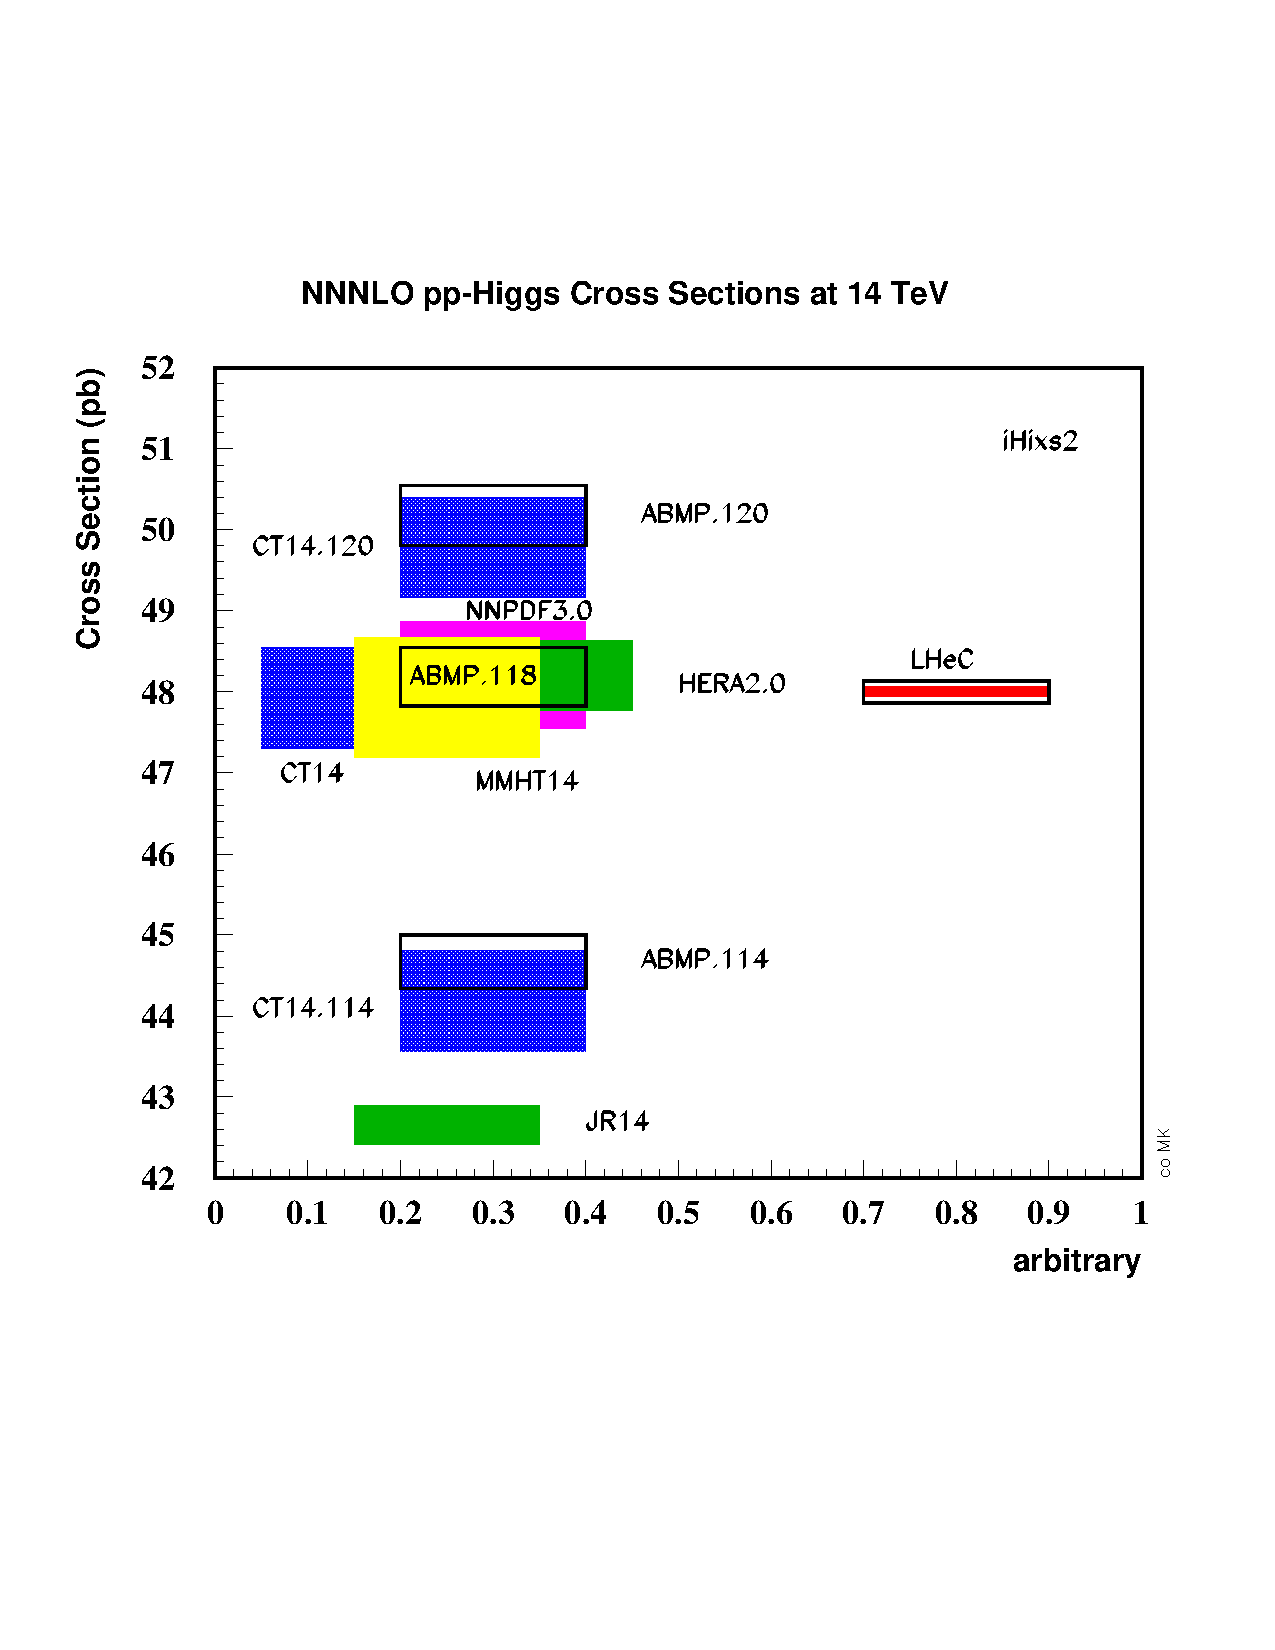
\includegraphics[width=1.0\textwidth]{Strong-Interaction/img/higgsPDF.pdf}
%\vspace{-5.cm}
%\caption{Cross sections of Higgs production calculated to N$^3$LO using the iHix program~\cite{Dulat:2018rbf} for existing PDF parameterisation sets (left side) and for the LHeC PDFs (right side).  The widths of the areas correspond to the uncertainties as quoted by the various sets, having rescaled the CT14 uncertainties from 90 to 68\,\% C.L. Results (left) are included also for different values of the strong coupling constant $\alpha_s(M_Z^2)$, from 0.114 to 0.120, see text. The inner LHeC uncertainty band (red) includes the expected systematic uncertainty due to the PDFs while the outer box illustrates the expected uncertainty resulting from the determination of $\alpha_s$ with the LHeC.}
%\label{fig:ihix}
%\end{figure}



%\subsubsection{The high-$\alpha_s$ or matter
%confined
%regime}
%\JDH{0.5p, plus a figure}}

%\begin{itemize}
%\item Key overall objectives.
%\item Experimental knowledge about QGP and theoretical progress. Impact on our understanding of strongly interacting systems in particle, nuclear, astro(particle) physics and cosmology.
%\item Main challenges, experimental and theoretical.
%\item \JDH{Urs will work on this}
%\end{itemize}
\subsection{Collective properties of QCD matter}
The Standard Model implies that our Early Universe has undergone a series of phase transitions of fundamental quantum fields. Specifically, for QCD, lattice calculations predict the transition of matter to a quark-gluon plasma (QGP) in which partons are deconfined and chiral symmetry is restored~\cite{Bazavov:2019lgz}. QCD is the only phenomenologically realised non-Abelian Quantum field theory whose high temperature phase is experimentally accessible in the laboratory~\cite{Citron:2018lsq}. Most generally, the focus of experimentation with nuclear beams is on learning how collective phenomena and macroscopic properties, involving many degrees of freedom, emerge under extreme conditions from the microscopic laws of Quantum Chromodynamics. This includes assessing thermal properties of QCD matter, characterising the QCD non-equilibrium dynamics that evolves nucleus-nucleus collisions towards equilibrium, quantifying the initial conditions of the collective dynamics, e.g.\ in terms of nuclear parton distribution functions, and establishing the system-size of collective phenomena from proton-proton ($pp$) via proton-nucleus ($pA$) to central nucleus-nucleus ($AA$) collisions as well as their dependence on centre of mass energy. 

In the soft (low-transverse momentum) sector, the occurrence of numerically large and abundant signatures of collectivity in $AA$ collisions is by now firmly established. In particular,  measured hadronic particle distributions show large flow-like momentum correlations that are in one-to-one correspondence with the initial spatial anisotropies in the collision system and that are thus unambiguous telltale signs of collective evolution. Also, soft particle distributions are found to approach hadrochemical equilibriumci~\cite{Andronic:2017pug}. Model comparisons support fluid-like behaviour of the system with close to minimal dissipative properties and statistical hadronisation. Similarly, the occurrence of numerically large jet quenching signals in all hard (high-transverse-momentum) hadronic observables is a generic feature of nucleus-nucleus collisions. These data indicate that nucleus-nucleus collisions evolve rapidly and efficiently towards equilibrium and that the detailed analysis of how hard out-of-equilibrium probes soften and isotropise, i.e.\ quench, can provide insight into the microscopic mechanisms underlying QCD equilibration phenomena. The discoveries of the LHC Run\,2 have added now a qualitatively novel dimension to these findings by establishing that smaller but non-vanishing flow-like signatures and medium-modified hadrochemical abundances persist in the smaller $pp$ and $pA$ collision systems, and that these signals of collectivity increase smoothly from minimum bias $pp$ to central $AA$ collisions. These qualitative phenomena cannot be accounted for in terms of physics effects commonly invoked for multi-particle production in $pp$ collisions, and they thus constitute a challenge for the understanding of both, $pp$ and $AA$ collisions. In contrast, unambiguous signatures of jet quenching have not yet been established in these smaller collision systems, though they may become accessible with refined measurements in the future. 

Capitalising on these previous discoveries, the experimental collaborations at the LHC and the world-wide theory community working on heavy ion phenomenology have identified  four major motivations for future experimentation with nuclear beams, namely~\cite{Citron:2018lsq} (see also Secs.~\ref{epcoll} and \ref{hot}): i) Characterising the long-wavelength properties of QGP matter with unprecedented precision, ii) probing the inner workings of the QGP, iii) developing a unified picture of particle production across system size and iv) exploring nuclear parton densities and searching  for a possible onset of parton saturation over a wide range of $(x,Q^2)$ are the four main themes along which experimentation with nuclear beams will be oriented  during HL-LHC. The generic denominator of these multiple studies is to arrive at a detailed, experimentally tested dynamical understanding of how out-of-equilibrium evolution occurs and equilibrium properties arise in a non-Abelian quantum field theory. 
\vfill

%%%%%%%%%%%%%%%%%%%%%%%%%%%%%%%%%%%%%%%%%%%%%%%%%%%%%%%%%%%%%%%%%%%%%%%%%%%%%%%%%
\section{Hadronic structure}
%\JDH{2.5p}} \JDH{editor: Ferenc}\\
%For each item we need the following %information: approved or foreseen timeline, %main objectives, experimental methodologies, %key challenges, required theory efforts and %methodology, estimate of the size of the %community involved or expected to be involved, %...

%\subsection{Ongoing experimental programmes \JDH{0.5p}}

%\begin{itemize}
%\item The need for a better understanding of the hadronic structure
%\item LHC experiments ($\alpha_s$, PDFs, text pQCD, non-perturbative QCD, %...)
%\item Experimental programmes with fixed-target experiments (high-x, ...)
%\item DIS experiments to test QCD
%\end{itemize}

%\subsection{Future experimental opportunities \JDH{2p}}

%\begin{itemize}
%\item Electron-proton collisions (LHeC, EIC, FCC)
%\item Electron-ion collisions (LHeC, EIC, FCC)
%\item Proton-proton collisions (LHC, HL-LHC, HE-LHC, % FCC)
%\item Fixed-target experiments (LHC, HL-LHC, COMPASS)
%\item Opportunities of HL-LHC beams after the regular %HL-LHC physics programme
%\item Synergies between these programmes
%\end{itemize}

%%%%%%%%%%%%%%
\subsection{QCD and collider experiments (LHC, HL-LHC, HE-LHC, FCC, CEPC)}
%%\subsubsection{Proton-proton collisions (LHC, HL-LHC, HE-LHC, FCC)}

Although QCD is not the main driving force behind future colliders, QCD is
crucial for many pp, ee measurements, both as signals and backgrounds. The
precision needed to fully exploit all future ee/pp/ep/eA/AA standard model and
BSM programs require exquisite control of perturbative and
non-perturbative QCD physics. There are unique QCD precision studies accessible
at FCC-ee, ILC,  CEPC-ee, the Super c-tau Factory (SCT@BINP), and at FCC-pp and CEPC-pp. The main
themes are detailed in the following.

The QCD coupling parameter $\alpha_s$ is the least-known coupling of the
standard model. Its value impacts all QCD cross sections and decays, it is
a leading parametric uncertainty (in some cases together with the charm
and bottom masses) in calculations of key quantities in Higgs, top quark, and
electroweak physics~\cite{dEnterria:2019its}, and
its energy evolution affects the range of stability of the electroweak vacuum
approaching the Planck scale.
% leading uncertainty in Higgs-, top and electroweak physics, also related to
% vacuum stability problems and the Planck scale.
Future colliders enable a per
mille precision determination of $\alpha_s$ via hadronic Z, W, and
$\tau$-decays, and jet shapes (FCC-ee, FCC-pp, SCT).
%
Parton distribution functions have a wide impact on new physics at high-$x$, as
well as on new QCD evolution at low-$x$. Experimental study of partonic
processes will provide key constraints and result in high-precision PDFs
(HL-LHC, HE-LHC, FCC-hh). Worth to note that FCC-ep is definitely required
to reach 1\% uncertainty for various cross section at FCC-pp.
%
FCC-ee provides multiple handles to study gluon radiation and gluon-jet
properties, as well as studies on jet substructure (N$^n$LO+N$^n$LL, see Sec. \ref{precision_sec}) and flavour
tagging through quark/gluon/heavy-quark discrimination, also giving access to
high precision parton fragmentation functions~\cite{Anderle:2017qwx}. FCC-pp enables unique studies of
highly-boosted dijets and multijets, as well as,  heavy flavours,  pentaquarks and other exotic hadron structures.
%
In the field of non-perturbative QCD, FCC-ee allows for a per cent-level
control of colour reconnection, while all machines give access to
high-precision measurements on hadronisation (baryon and strangeness
production, final-state correlations, bound states).

%%%%%%%%%%%%%%

%%%%%%%%%%%%%%
\section{Electron-proton collisions (LHeC, EIC, FCC)}
\label{epcoll}

Deep inelastic lepton-nucleon scattering is a powerful and unique tool to study
nucleon structure and unravel QCD with high precision data and on firm
theoretical grounds. The future of DIS is bright with two proposed independent,
high luminosity electron-hadron colliders. DIS collider measurements extend substantially the
kinematic range of fixed target lepton-hadron scattering experiments. Excellent
precision is achieved through the redundant reconstruction of the leptonic and
hadronic final states while theoretically a next order of perturbation theory
in QCD and EW has to be controlled. Tagging of photons, electrons, protons, and
neutrons near the beam pipe as well as tagging of heavy flavour decays in a
large rapidity range will be special experimental challenges.

At medium energies, below that of HERA, a US-based electron-ion collider\footnote{At the time of writing, DOE is moving forward to approve the
Mission Need soon, and has organised a panel to assess options for siting and
consideration of best value between the two proposed concepts~\cite{Hallman:2019}.} (20 to
140 GeV c.m.\ energy) and a Chinese EIC (electron ion-collider, 16 to 34 GeV) will study the polarised
nucleon structure, this way contributing to the solution of the nucleon spin
puzzle, and explore the structure of the proton in three-dimensions at medium
and high $x$.

At the energy frontier, the CERN-based hadron-electron colliders (LHeC,
FCC-eh), with c.m.\ energies above that of HERA, will resolve the flavour
structure of unpolarised nucleons from $x$ about 10$^{-6}$ to near 1, measure
$\alpha_s(m_\text{Z})$ at third order perturbation (N$^3$LO) to per mille accuracy, and
discover new parton dynamics (gluon saturation). The LHeC and FCC-eh are precision
Higgs- and EW-physics facilities with a remarkable BSM discovery potential. The $ep$ c.m.\ energies are 1.3~TeV for LHeC using
7~TeV $p$ from HL-LHC, and 3.5 (2.2)~TeV for FCC-eh using 50 (20)~TeV $p$ from
FCC-hh. The high-energy electron beams are produced using novel energy recovery
acceleration techniques (ERL), transforming the hadron colliders into an $eh$ and
$hh$ twin collider complex. Such a synergy will establish physics programmes
reaching much further than those of the HL-LHC and of future $hh$ colliders alone.

%%%%%%%%%%%%%%
\begin{figure}

 \centering
 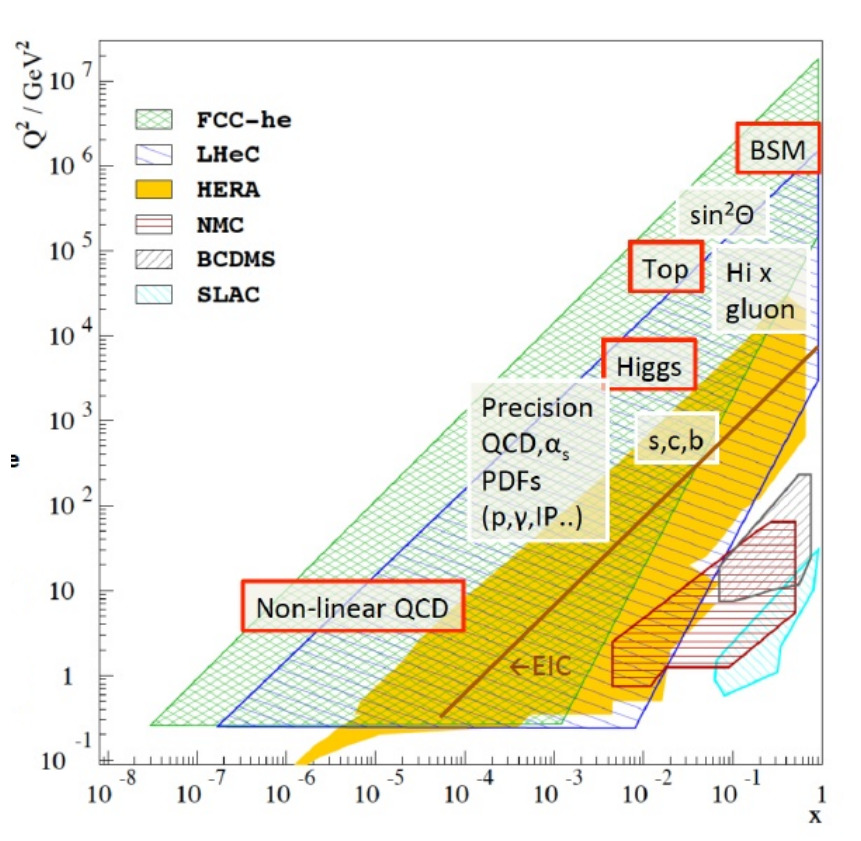
\includegraphics[width=0.49\textwidth]{Strong-Interaction/img/britzger_dis2017.jpg}
 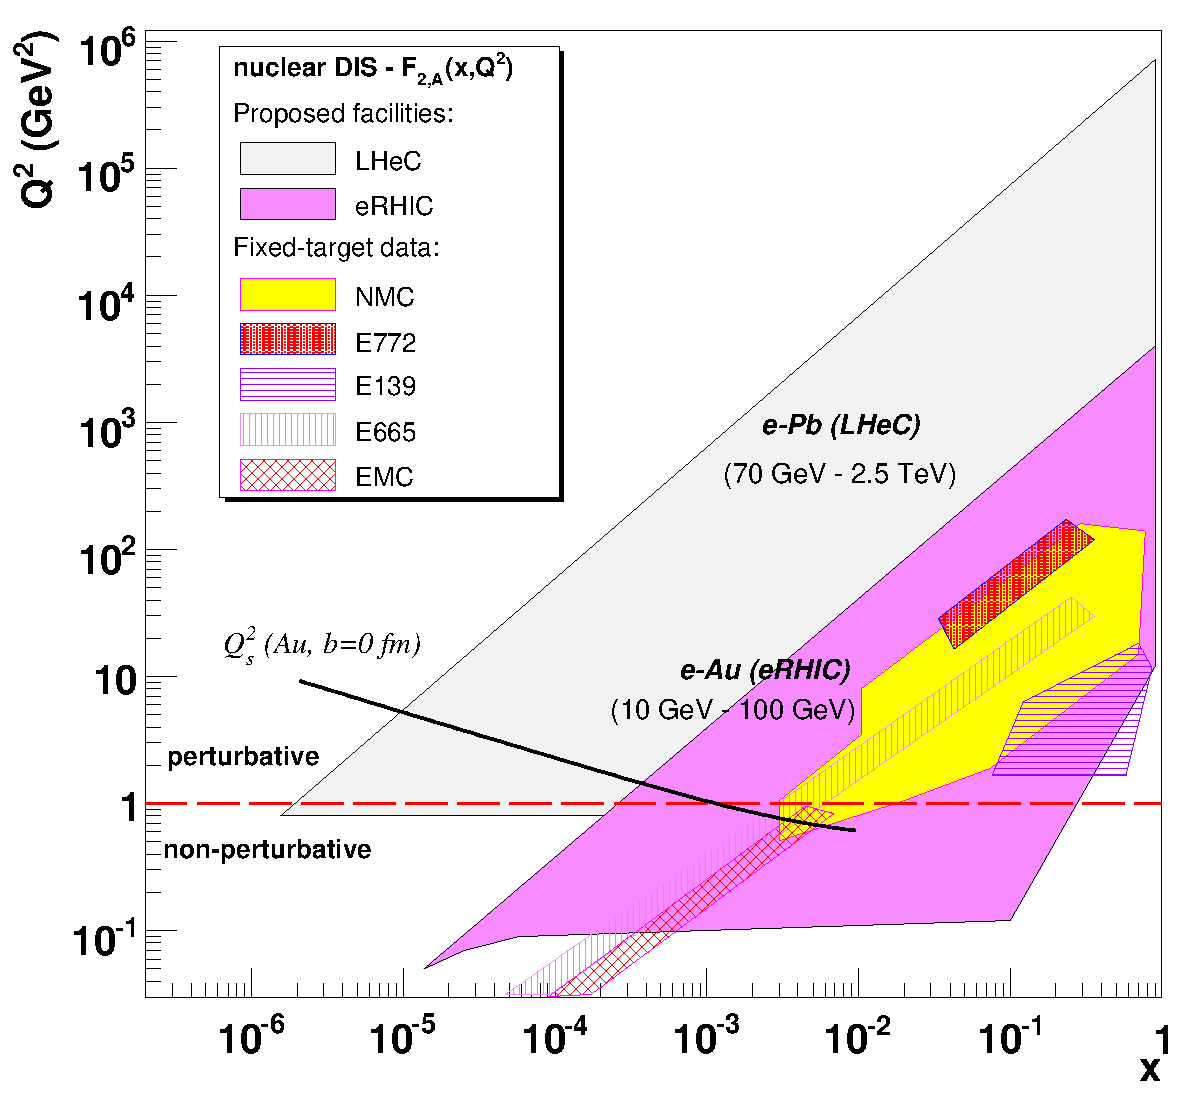
\includegraphics[width=0.49\textwidth]{Strong-Interaction/img/denterria_nDIS_x_Q2_map_future.pdf}

 \caption{Kinematic $(x, Q^2)$ plane probed in $e-p$ (left) and $e-A$ processes
(right): existing data compared to proposed particle and nuclear DIS
facilities~\cite{Britzger:2017,dEnterria:2007jwb}.}

 \label{fig:xQ2}

\end{figure}
%%%%%%%%%%%%%%

%%%%%%%%%%%%%%
\subsection{Electron-ion collisions (LHeC, EIC, FCC)}

Several electron-ion ($eA$) colliders with per nucleon luminosities $\sim
10^{33}-10^{34}~\mathrm{cm^{-2}s^{-1}}$ are projected to start operating in the
2030s.
%%%%
%With c.m.\ energies of $0.8-2.2$~TeV/nucleon, the
%LHeC/FCC-eh~\cite{AbelleiraFernandez:2012cc,Benedikt:2018csr} extend the
%kinematic reach of available DIS data by $3-5$ orders of magnitude. %
Colliding
electrons from an ERL with the HL-LHC or FCC nuclear beams, the LHeC is the
most powerful $eA$ facility that one can build in the next decades. It will
clarify the partonic substructure and dynamics in nuclei in an unprecedented
kinematic range. Also, it will unequivocally probe the new non-linear partonic
regime of QCD through density effects in $ep$ and $eA$, that increase both with
$1/x$ and mass number $A$. The LHeC will provide an accurate benchmark for perturbative probes,
the initial conditions for collective expansion, for the understanding of the
prior dynamics and the collective behaviour  in $pp$ and $pA$ collisions.
%, and for
%elucidating the QCD origin of the quark-gluon plasma state.

The EICs in the US~\cite{Accardi:2012qut} and China~\cite{Chen:2018wyz}, with
c.m.\ energies below 100~GeV/nucleon, are dedicated to a detailed mapping of
nuclear structure and its $A$ dependence in the medium $x$, lower $Q^2$ region,
extending the kinematic $(Q^2, 1/x)$ range as compared to existing DIS data by
up to a factor of 30. The flexible choice of lower energy, while limiting
access to small $x$, is optimal for pursuing a unique proton (and light ion)
spin programme.
%aimed at resolving the long-standing nucleon spin puzzle.

The development of a broad QCD programme for the 2030s developing the synergies
and complementarities between different machines and collision systems,
$pp/pA/AA$ and $ep/eA$, should be encouraged.


\subsection{Fixed-target experiments (LHC, HL-LHC, SPS M2 beamline)}

The multi-TeV LHC proton- and ion-beams allow for the most energetic
fixed-target (LHC-FT) experiments ever performed opening the way for unique
studies of the nucleon and nuclear structure at high $x$, of the spin content
of the nucleon and of the nuclear-matter phases from a new rapidity viewpoint
at seldom explored energies~\cite{Brodsky:2012vg,Hadjidakis:2018ifr}.

On the high-$x$ frontier, the high-$x$ gluon, antiquark and heavy-quark content
(e.g.\ charm) of the nucleon and nucleus is poorly known (esp. the gluon PDF for
$x \gtrsim 0.5$). For instance, the gluon EMC effect should be measured to
understand that of the quarks. Such LHC-FT studies strongly connect to
high-energy neutrino and cosmic-ray physics.

The dynamics and spin of gluons and quarks inside (un)polarised nucleons is
also very poorly known; possible missing contributions are expected to come
from their orbital angular momentum. The LHC-FT mode enables to test the QCD
factorisation framework and to measure transverse-momentum-dependent
distributions, such as that of the linearly polarised gluons in unpolarised
protons or the correlation between the proton spin and the gluon transverse
momentum.

For heavy-ion studies, the proposed fixed-target experiments with LHCb and
ALICE enable the exploration of new energy regimes between SPS and RHIC
energies, across a wide rapidity domain to scan azimuthal asymmetries, and the
use of new physics probes (e.g.\ excited quarkonia, Drell-Yan pairs to test the
factorisation of nuclear effects).
%
In addition, double crystal LHC-FT experiments give access to studies beyond
QCD, such as magnetic and electric dipole moments of heavy baryons.
 
There are two proposed ways towards LHC-FT collisions: a slow extraction with a
bent crystal, or internal gas target inspired by SMOG@LHCb, Hermes, H-Jet,
and others. The physics reach of the LHC complex can greatly be extended at a
very limited cost with the addition of an ambitious and long term LHC-FT
research program. The efforts of the existing LHC
experiments to implement such a programme, including specific R\&D actions on the
collider, deserve support.

The CERN M2 beamline also allows for further dedicated nucleon-spin analyses
and innovative studies of the kaon structure (gluon content, spectroscopy,
polarisability, etc.).

%%%%%%%%%%%%%%
\subsection{Opportunities of HL-LHC beams after the regular HL-LHC physics
programme}

% The regular HL-LHC programme [Id152] is expected to start in 2026 and last
% for at least ten years of operation. In the end, the HL-LHC will have
% produced a wealth of data on pp, pA and AA collisions. This data will
% constrain the parton densities in a region of $x$ from the valence region
% down to $10^{-4}$ with a statistical accuracy of a few per cent [5].
% Approximately the same range in $x$ is expected to be covered by the
% Electron-Ion Collider (EIC) [Id103,Id99,Id74] with c.m.\ energies between
% 20-140 GeV that could run in parallel in the US. Many open questions about
% the nonlinear QCD effects of the saturation region at very small $x$ will
% likely remain, requiring future higher energy machines.

The proposed LHeC
%[Id159,Id103]
with a c.m.\ energy of 1.3~TeV will allow
high-precision measurements of the parton densities from high $x$ down to $x
\sim 10^{-6}$. It will be in operation at the earliest around 2030, but if not
realised during the regular HL-LHC programme, it could be an opportunity for
continued use of the HL-LHC beams afterwards. If in the future (beyond 2040) a
27~TeV c.m.\ energy HE-LHC
%[Id160]
or an FCC-hh is realised, the corresponding
LHeC or FCC-eh
%[Id135,Id103] 
will have a c.m.\ energy of several TeV, enhancing
the kinematic reach further. Even higher energy electron-proton collisions may
be reached if in the future LHC-proton driven plasma wakefield accelerated 3
TeV electrons can be realised and collided with LHC protons. Such a 9~TeV
collider, called VHEeP (AWAKE++),
%[Id58,Id103], 
will probe $x$ down to an
unprecedented $10^{-8}$. However, the target luminosity of
$10~\mathrm{pb^{-1}}$ over the entire lifetime is modest, so it should not be
viewed as a substitute for a high precision machine like the LHeC. This also
applies to the SPS-driven Plasma Electron-Proton/Ion Collider (PEPIC) 
%[Id58],
that will have a c.m.\ energy of 1.4~TeV, but a luminosity several orders of
magnitude lower than LHeC.

The region of large $x$, which is relevant for searches for new massive BSM
particles at the LHC and interesting for the nuclear dependence of the gluon
distribution, will not be covered by HL-LHC or EIC either, but can be covered
by the LHeC and/or by fixed-target (FT) experiments,
%[Id47,Id67], 
either during
the regular HL-LHC programme or afterwards. FT experiments at an HE-LHC would
have a relatively modest increase in c.m.\ energy from 115 GeV to 163 GeV.

%%%%%%%%%%%%%%
\subsection{Synergies between these programmes}

There are a number of striking synergy examples among future QCD physics
experiments:

\begin{itemize}

\item The determination of the strong coupling constant at per mille level
with LHeC/FCC-eh, FCC-ee, CEPC  and lattice gauge theory will lead to a new level of
understanding of QCD and to confidence in its predictive power. Agreement at
this high level of precision is required but will not likely result from the
first attempts in either of the above three directions.
% Rather, this is a programme to develop QCD much further and to test its embedding in a grand unified theory.

\item Precision measurements of flavour-separated parton distributions and the
correct theoretical description of the partonic contents of the proton is a
necessity for precision physics and searches for new physics with the LHC and
subsequent higher energy hadron colliders. It can be provided to the required
accuracy and kinematic range only by a TeV ep collider with a factor of 100
higher luminosity than that of HERA. Independent input on PDFs empowers e.g.\
precision interpretations within contact interaction and effective field theory
frameworks but also in the understanding of QCD background processes for e.g.\
novel SUSY searches.

\item It is essential to perform spin studies both at pp and ep machines to test
pQCD predictions with a sign change in some spin asymmetries.

\item The characterisation of the quark-gluon plasma suffers from  sizeable
uncertainties e.g.\ from our lack of knowledge of nuclear PDFs for quarkonium
suppression~\cite{Andronic:2015wma} and  charm production cross section in $AA$ collisions~\cite{Andronic:2017pug}  or of the initial conditions for collective
expansion for the extraction of the QGP transport
coefficients~\cite{Niemi:2015qia,Schenke:2012wb}, and of the role of parton fragmentation and hadronisation in cold nuclear
matter~\cite{Accardi:2009qv}. Therefore, it requires novel
input on nuclear parton structure, on nuclear multiparton correlations, on parton
fragmentation and hadronisation in-vacuum and in cold nuclear matter, which
% nuclear structure, on nuclear binding effects, on fragmentation and
% hadronisation information which
should come from future electron-ion and
electron-positron colliders. The observation of long-range correlation effects
even in $pA$ collisions demands a detailed investigation of the lightest systems,
$ep$ and $eA$.

\item The development of accelerator technology (energy recovery) for a next
energy frontier ep collider is supported by and also invites low energy ERL
facility developments. These have fundamental low energy physics programmes, in
particle and nuclear physics. Intense $\sim$1~GeV electron ERL facilities have
a wide range of important applications for material-, bio-, accelerator science,
and other branches of science and technology. The high-quality requirements for
superconducting radio frequency are synergetic with developments of
electron-positron colliders. The first 802~MHz cavity, for example, has been
developed jointly for LHeC and FCC-ee, by CERN and JLab.

\end{itemize}

%%%%%%%%%%%%%%%%%%%%%%%%%%%%%%%%%%%%%%%%%%%%%%%%%%%%%%%%%%%%%%%%%%%%%%%%%%%%%%%%%
\section{Hot and dense QCD}
\label{hot}
%\JDH{2.5p}} \JDH{editor: Anton}\\
%For each item we need the following information: approved or foreseen timeline, main objectives, experimental methodologies, key challenges, required theory efforts and methodology, estimate of the size of the community involved or expected to be involved, ...

The study of hot and dense QCD matter is performed over a broad range of energies, both in fixed-target and collider experiments.
%At high energies, a deconfined state, called the Quark-Gluon Plasma (QGP), is formed; according to the standard Big Bang model, the QGP was a state of our Universe until about 10 $\mu$s in its evolution. 
The connection to theory is achieved via the LQCD formalism, hydrodynamic description, microscopic transport models and statistical models.
In this latter case, an illustration is given in Fig.~\ref{fig:Tmub} of the results achieved to date about the phase diagram of QCD, where the points extracted from fits of hadron yields with the statistical hadronisation (thermal) model, describing the chemical freeze-out - which, at higher energies, $\mu_B\lesssim$ 300 MeV, appears to coincides with the chiral crossover phase boundary as determined in LQCD.
Whether a critical point and a first order phase transition exist in this phase diagram is currently a subject of intense research.

\begin{figure*}[!ht]
\center
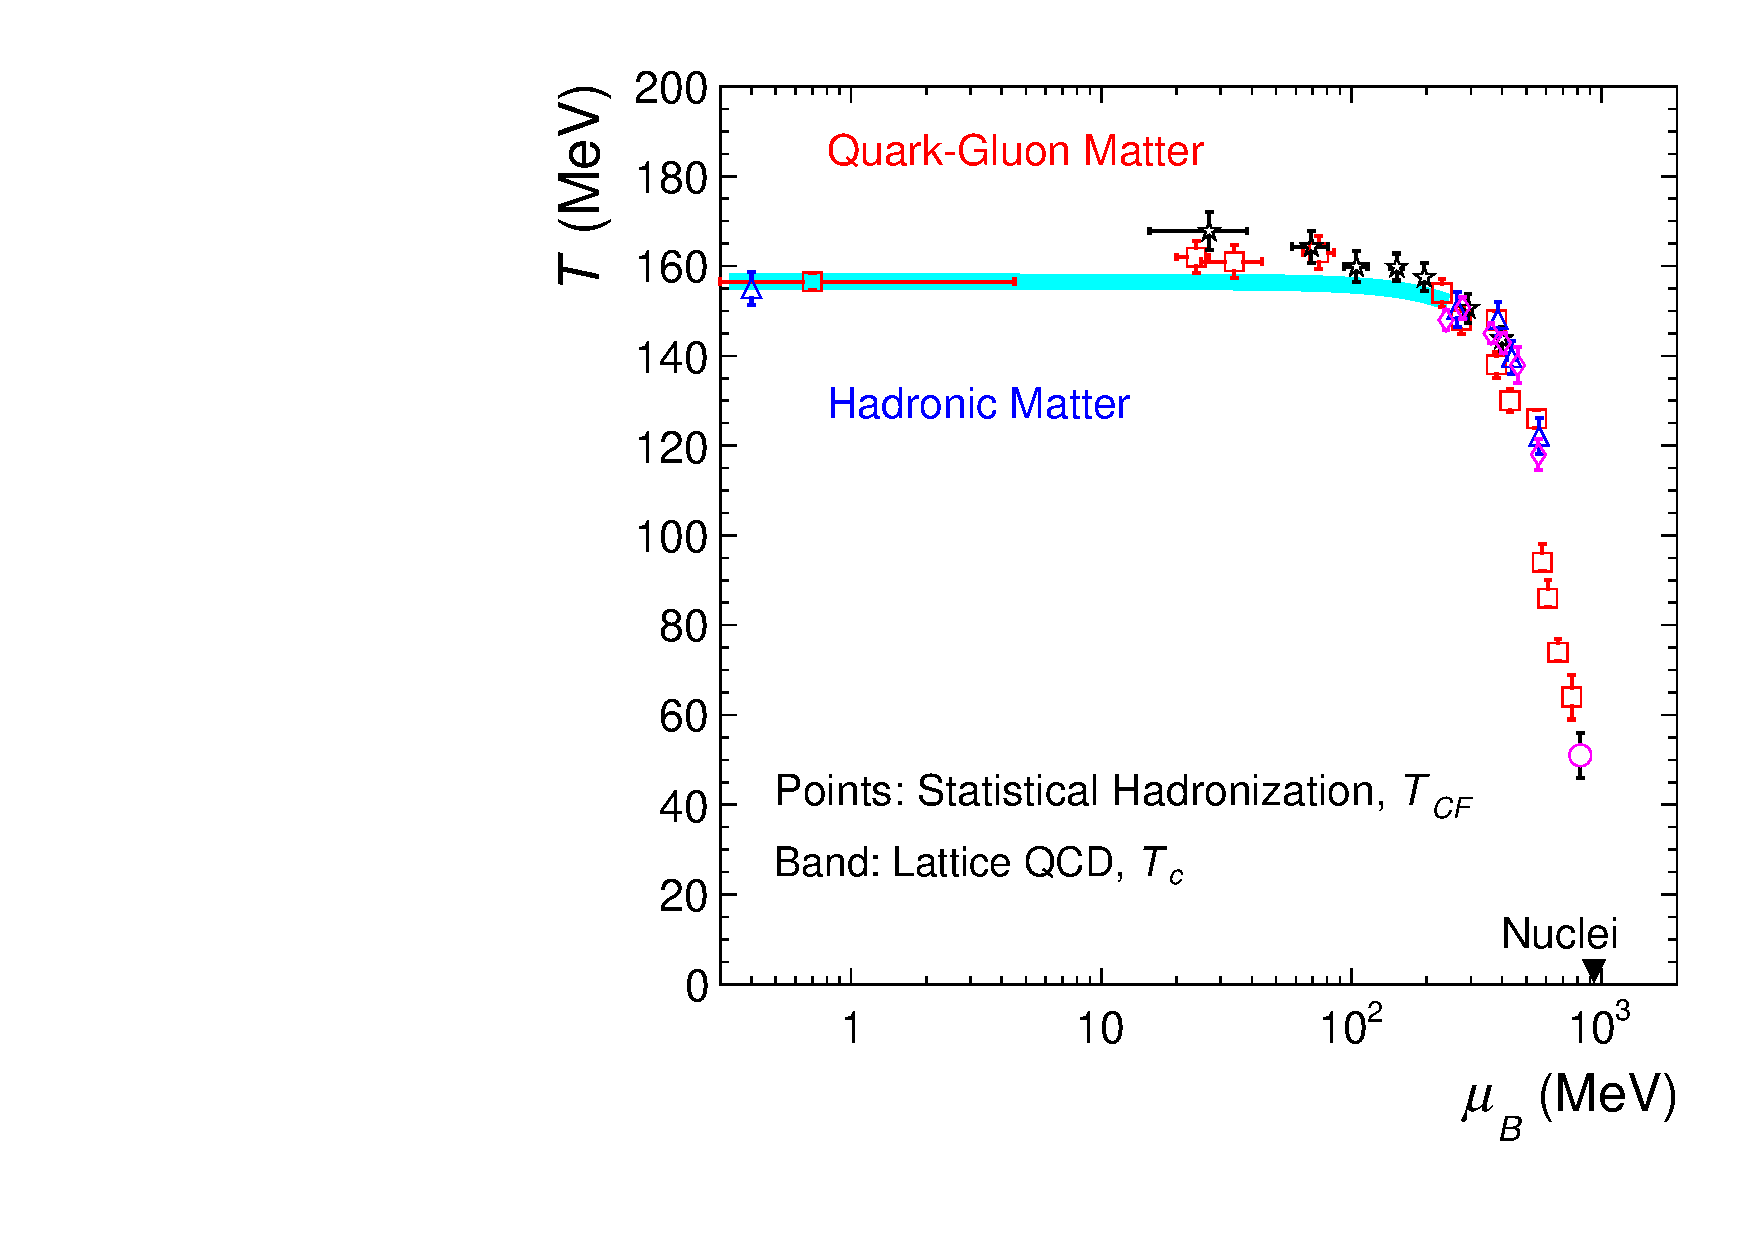
\includegraphics[width=3.355in]{Strong-Interaction/T-mub_2019.pdf}
 \caption{The QCD phase diagram in the temperature - baryochemical potential plane. The band is from LQCD calculations~\cite{Bazavov:2018mes}, the points from statistical hadronisation model fits to hadron yields in heavy-ion collisions over a broad range of collision energy (updated from ref.~\cite{Andronic:2017pug}).}
\label{fig:Tmub}
\end{figure*}

A multitude of observables, like photon and dilepton yields, jets, heavy quarks, correlations and fluctuations, help to quantitatively describe the dynamics and the properties of the hot and dense matter.
Also a subject of intense research is currently the question of the formation in high-multiplicity proton(deuteron)-nucleus (or even proton-proton) collisions of a droplet of deconfined matter that expands collectively, akin to the observations in nucleus-nucleus collisions.

\subsection{The ongoing experimental programme of relativistic heavy-ion collisions}
%\JDH{0.5p}}

A very successful data taking for heavy-ion collisions in Run 2 at the LHC was completed, with Pb--Pb collisions at a nucleon-nucleon c.m. energy $\sqrt{s_{\mathrm{NN}}}$ = 5.02 TeV and $p$--Pb collisions at $\sqrt{s_{\mathrm{NN}}}$ = 5.02 and 8.16 TeV, recorded by all four experiments: ALICE,  ATLAS, CMS, and LHCb, with luminosities exceeding the initial goals.
The first physics results in a fixed-target mode were recently reported by the LHCb collaboration~\cite{Aaij:2018ogq,Aaij:2018svt}.

At BNL data taking is ongoing with the STAR experiment at RHIC in the beam energy scan (BES-II) program, spanning $\sqrt{s_{\mathrm{NN}}}$ = 7.7 - 62 GeV in Au--Au collisions. At CERN,  the SPS programme is ongoing, with data taking in various collision systems at $\sqrt{s_{\mathrm{NN}}}$ = 7 - 17 GeV with the NA61/SHINE fixed-target experiment, which provides as well important measurements for neutrino oscillation experiments.
At the SIS18 at GSI, the HADES experiment continues to take data at $\sqrt{s_{\mathrm{NN}}}\simeq$ 2.5 GeV, while at JINR the BM@N detector is in operation at the Nuclotron in a similar energy range, currently with light ions \cite{Galatyuk:2019lcf}.

\subsection{The future opportunities for experiments at high-energy colliders}
%\JDH{1p}}

The ongoing and foreseen upgrades of the 4 detectors at the LHC will meet the challenge of providing the required detector performance for the data taking with ion collisions with HL-LHC in Runs 3 and 4, a physics programme that is approved and will bring a significant advance in the field for the next decade~\cite{Citron:2018lsq}. 
The focus is on rare and challenging observables of the hot and dense phase, that could only be glimpsed with the existing data. Those include:
i) thermal radiation (photons and dileptons), to characterise the electromagnetic emissivity;
ii) heavy flavour baryons  and (hyper)nuclei, to study in detail the hadronisation, on which the complex objects shall give unique insight; 
iii) quarkonium, both in the charm and beauty sector, to pin down quantitatively the basic mechanism of colour screening in QGP and the dynamics of (re)generation or quarkonia in QGP and at the QCD phase boundary;
iv) fluctuations of conserved charges, to establish experimentally signatures of the phase boundary that are predicted by solving QCD on the lattice;
v) highly energetic jets, to probe extreme regimes of parton energy loss (jet quenching) in QGP.
Together, this suite of observables, will provide new insights and a precise characterisation of the QGP (via transport coefficients) in the highest temperature and density regime. 

Beyond Run 4, a proposal for a next generation experiment at the LHC has been put forward~\cite{Adamova:2019vkf} to address hot QCD
physics, where the QGP initial temperature $T_{in}\sim 0.5$ GeV,   and soft  QCD   at very low $p_T< 10$  MeV/c, (while the particle physics experiments could continue data taking with heavy ions with focus on the hard regime). Advances in detector technology, for instance the possibility to curve thin silicon wafers, will open up the possibility to build a very light detector, enabling to reach very soft probes, both with hadrons and with dileptons, to probe in a direct way the quantum nature of the dense QGP state.
%
In addition, a complementary proposal has been
also presented to use in parallel the ATLAS, CMS and LHCb experiments in unique
BSM searches accessible in the high-luminosity ion-ion mode beyond
Run-4~\cite{Bruce:2018yzs}. In this time span, a complete FT-LHC program could also be realised with the ALICE and LHCb detectors in parallel to these measurements.

Advances in detector technology will be equally relevant for the FCC, where an attractive physics programme is envisaged~\cite{Dainese:2016gch}. The motivation for the FCC lies primarily in the unique availability of hard probes, enabled by the significant increase as a function of energy of their production cross section. Examples include beauty quarks, whose thermalisation in QGP can be determined, or top quarks, whose (boosted) decay to jets will provide a unique handle on the tomography of QGP. That goal could be realised, albeit in a less significant way, also at the HE-LHC.
Both at the FCC as in the HL(HE)-LHC a significant gain in luminosity can be achieved with lighter ions, which consequently may be more advantageous for rare observables. Collisions of protons with nuclei are part of the heavy-ion programme at HL(HE)-LHC and are envisaged too for the FCC~\cite{Abada:2019lih}.

It is important to notice that, at high-energy colliders, colliding heavy ions provide a significant photon flux, enabling unique studies of cold QCD matter in the regime of high gluon occupancy (low Bjorken $x$); for instance, exclusive photoproduction of J/$\psi$ at FCC can probe down to $x$=10$^{-7}$.
Such photon-photon or photon-induced collisions, already now providing interesting results at the LHC, have also the potential to bring sensitivity to BSM physics, providing discovery  potential (or exclusion limits) for magnetic monopoles or axions~\cite{Bruce:2018yzs}.
Ultra-strong transient (short-lived) magnetic fields are created in heavy-ion collisions and are probed via particle correlations which may provide insights relevant for astrophysics.
The high production rates of multi-strange hyperons at collider energies enables the study of their interaction properties, with results of relevance for the understanding of the neutron star structure, while abundantly-produced antimatter is of relevance for antimatter search in the Universe (currently with the AMS detector).

The long-term measurements in heavy-ion collisions will benefit from a sustained support from the theory community. The continuous improvement of existing theoretical tools and models, as lattice QCD or hydrodynamics, as well as the development of new techniques, in particular calculations in higher orders, will be crucial for the characterisation of QGP in its regime of highest temperature and densities.

This expected progress, both experimental and theoretical, will impact and benefit from the experiments in the next decade(s) at lower energies at RHIC (STAR and sPHENIX experiments) and at the NICA collider under construction at JINR, which will provide beams spanning $\sqrt{s_{\mathrm{NN}}}$ = 4 -- 12 GeV, with the MPD experiment planned to start operation in stages in 2022.

\subsection{The future opportunities for fixed-target experiments} %\JDH{1p}}

The RHIC fixed-target program, planned to start in 2020, will cover $\sqrt{s_{\mathrm{NN}}}$ = 3.0 -- 7.7 GeV, corresponding to $\mu_B\simeq$ 400--700 MeV. 
The approved FAIR accelerator will deliver high-intensity beams ($\sqrt{s_{\mathrm{NN}}}$ up to 5 GeV) starting in 2025; the CBM detector aims at a collision rate of 10 MHz with continuous readout and online tracking and event selection. 
The  NA61/SHINE experiment at SPS, currently being upgraded with vertex capability (used are pixel sensors developed for ALICE), will extend in the coming years its suite of observables into the charm sector.
An experiment at the SPS (NA60+) dedicated to thermal dimuon, open and hidden charm measurements is curently under design and aims at collision rates of 10 MHz~\cite{Dainese:2019xrz}.
A heavy-ion programme with similar characteristics as that at FAIR is currently being prepared for the J-PARC facility.
The physics motivation \cite{Friman:2011zz} is common for all these fixed-target experimental programs and it is shared as well by the BES programme at RHIC and by the NICA program~\cite{Ablyazimov:2017guv,Bzdak:2019pkr}.
It is the investigation of hot and compressed baryon-rich matter, with special focus on the discovery of the critical point and (consequently) of a first order phase transition in the QCD phase diagram. Also prominent is the determination of the Equation of State of compressed baryonic matter, which is of relevance for neutron stars and for neutron star collisions.
This will be achieved with correlations and fluctuations observables and with rare probes like dileptons, multi-strange hyperons or hypernuclei, probes that will become for the first time available (with abundant statistics) for this energy regime.

The highest-energy fixed-target programme can be realised with LHC beams~\cite{Hadjidakis:2018ifr}, both in the ALICE and LHCb experiments. The hot QCD component of such a programme has as a special aspect the broad coverage in rapidity which is also of relevance as input for cosmic ray physics.
%%%%%%%%%%%%% Krzysztof
%%%%%%%%%%%%%%%%%%%%%%%%%%%%%%%%%%%%%%%%%%%%%%%%%%%%%%%%%%%%%%%%%%%%
\section{Precision QCD}
\label{precision_sec}
%\JDH{1.5p}} \JDH{editor: Krzysztof}\\
%{\it For each item we need the following information: approved or foreseen timeline, main objectives, experimental methodologies, key challenges, required theory efforts and methodology, estimate of the size of the community involved or expected to be involved, ...}

%The  LHC experiments    have collected  a wealth of data with an unprecedented level of precision. The huge statistics  expected at the  HL-LHC will lead to an extension of the kinematic coverage of  relevant  measurements as well as to an improvement in their statistical and systematic uncertainties. Consequently,

As already introduced    in Sect.~\ref{section_low}, the  interpretation  of LHC data and the searches for new physics 
requires increased efforts to reach a higher level of precision and accuracy in key
theoretical predictions.
 This is the case in both the electroweak and the
   QCD  sectors of the Standard Model~\cite{Azzi:2019yne,Citron:2018lsq}.

% At the LHC, due to  the collinear factorisation theorems,  
The  QCD predictions for a scattering process,  owing to  the collinear factorisation theorems and universality,  are obtained by convoluting a perturbative 
scattering amplitudes        with the 
parton distribution functions,  (PDFs). Consequently, to reach sufficiently  high   accuracy in theoretical predictions  of strong interaction processes  good control of     partonic   cross sections,  the value of the  strong coupling constant $\alpha_s$,  and  the    precise determination of PDFs is required.

Detailed modelling of strong interactions also requires understanding how the partonic final state in hard scatterings evolves to the hadrons observed in the experiment. The quantitative description of  fragmentation and  hadronisation  is a part of the physics programmes at  fixed target and beam-collider experiments.

%%%%%%%%%%%%%%%%%%%%%%%%%%%%%%%%%%%%%%%%%%%%%%%%%%%%%%%%%%%%%%%%%%%%%%%%%%%%%%%%%
%%%%%%%%%%%%%%%
\begin{figure}[hbt]
 \centering
\includegraphics[scale=0.78]{Strong-Interaction/2matched_fixed-order_nnlo}
% \includegraphics[width=\columnwidth]{2matched_fixed-order_nnlo}
 \caption{Comparison among the matched normalised distributions  at:  N$^3$LL+NNLO, NNLL+NNLO, and the pure NNLO of the Higgs-boson transverse-momentum spectrum at the LHC~\cite{Bizon:2017rah}.  }
 \label{NLL}
\end{figure}
%%%%%%%%%%%%%%%%
%%%%%%%%%%%%%%%%%%%%%%%%%%%%%%%%%%%%%%%%%%%%%%%%%%%%%%%%%%%%%%%%%%%%
%%%%%%%%%%%%%
Some non-perturbative aspects  of QCD are  directly  accessible in   first-principles
calculation by formulating QCD on the lattice and  solving it numerically. LQCD provides quantitative input on hadron structure and spectroscopy,  the properties  of matter  under extreme conditions and  hadronic  contributions  to the processes and matrix elements relevant for the  SM and BSM~\cite{Aoki,Cirigliano:2019jig,Bazavov:2019lgz,Lehner:2019wvv,DeGrand:2015zxa}


\subsection{Methods and tools}
%\JDH{1.5p, each item around 8 lines}} \JDH{editor: Krzysztof}\\
%{\it Experimental measurements will be key to guide us to new physics. In order to make these precise measurements useful for a precise exploration, we need dedicated methods and tools. Effective Field Theories, PDFs/TMDs/GPDs, generators, $N^MLO$ calculations, lattice, non-perturbative models, etc. Indicate where and how support is required for the theory community, and motivate the need to foster collaboration between experimental and theoretical inclined researchers.}

At  parton level, QCD cross sections at high momentum scales $Q$  are obtained through perturbative series expansion in the strong coupling $\alpha_s(Q)$.
This is the most  straightforward and successful approach that is also systematically improvable in accuracy  by calculating an increasing number of coefficients in the series. The current standard of such calculations is the next-to-next-to-leading order (NNLO) accuracy~\cite{Boughezal:2015dva,Ridder:2015dxa,Czakon:2015owf,Czakon:2016dgf,Currie:2013dwa,Currie:2016bfm}.  However, in view  of high quality data at  LHC  and the expected high precision  measurements at HL-LHC,    there is a continuous theoretical  demand and efforts to go beyond NNLO and calculate QCD processes at the next-to-next-to-next-to-leading order, N$^3$LO.
   At present, the   hadron collider observables for which N$^3$LO QCD corrections have been calculated are e.g.\ the total cross section for Higgs boson production in gluon fusion~\cite{Anastasiou:2015ema,Mistlberger:2018etf} and in vector boson fusion~\cite{Dreyer:2016oyx}.
   Under QCD factorisation, the resulting predictions carry a residual uncertainty and dependence on the factorisation scheme due to the missing N$^3$LO (i.e., four-loop) splitting functions, recently motivating the computation of the QCD splitting functions at four loops \cite{Baikov:2006ai,Velizhanin:2011es,Baikov:2015tea,Davies:2016jie,Moch:2017uml}.  Furthermore, first steps have been taken towards more differential observables by computing  N$^3$LO  rapidity distribution of the Higgs boson at the LHC   in  gluon  fusion~\cite{Dulat:2017prg,Dulat:2018bfe,Cieri:2018oms}.  Moreover, fully differential distributions of jet production in deep inelastic scattering have been also derived    to N$^3$LO~\cite{Currie:2018fgr}.

Extending the perturbative  expansion  of QCD    to  the higher order is theoretically challenging as it    implies developing new methods and techniques to achieve the cancellation of infrared   divergences. At the NLO order there  are well established subtraction schemes and there are methods developed recently for NNLO calculations
\cite{Catani:2007vq,Bozzi:2005wk,Bonciani:2015sha,Boughezal:2015eha,Gaunt:2015pea,Czakon:2011ve,Boughezal:2011jf,Cacciari:2015jma,Ger}. %,Antena:mehod}.




In general,  N$^{\rm n}$LO  perturbation theory   is based on the expectation  that  calculating   a finite number of terms in the perturbative expansion is sufficient  since higher-order terms get progressively smaller and can be neglected once the desired accuracy is reached.  Thus, N$^{\rm n}$LO refers to calculations  of  cross sections $\sigma_{{\rm N}^{\rm n}{\rm LO}}$   which differ from their exact  value $\sigma_{ex}$, as  $\sigma_{ex}/\sigma_{{\rm N}^{\rm n}{\rm LO}}-1\sim \alpha_s^{{\rm n}+1}$.    In some processes, however,  logarithmically  (L) large  contributions appear at all orders  and spoil the convergence of the perturbative expansion.  In such cases,  it is necessary to rearrange   the perturbative expansion and perform resummation of these large logarithms to  all-orders in the perturbation theory.
Resummed calculations are typically needed in processes which depend on more than one scale,  and   L-terms are sensitive to the ratio of these scales. The numerical size of  logarithms can be of  order $L\sim 1/\alpha_s$. The  N$^{\rm n}$LL  accuracy of a resummed calculation  implies that, $\log(\sigma_{ex}/\sigma_{{\rm N}^{k{\rm LL}}})\sim \alpha_s^{n}L^{m}$, for  $m\geq n+1-k$  and  $L \gg 1$. Thus,  leading logarithm  (LL) terms are of order $1/\alpha_s$, NLL  of order 1 and   NNLL  of order $\alpha_s$.
%%%%%%%%%%%%%%%%%%%%%%%%%%%%%%%%%%%%%%%%%%%%%%%%%%%%%%%%%%%%%%%%%%%%%
\begin{figure}[t]
\begin{center}
  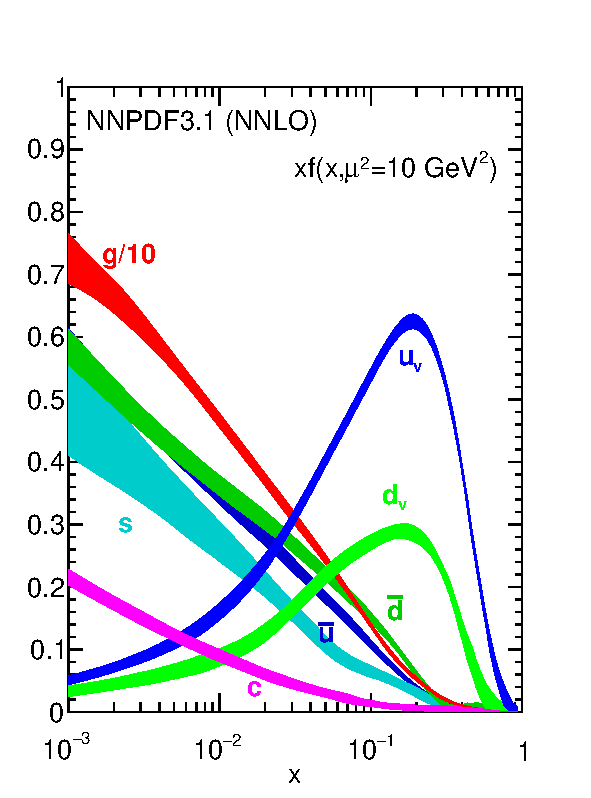
\includegraphics[scale=0.65]{Strong-Interaction/nnpdf31nnlo-10.pdf}
  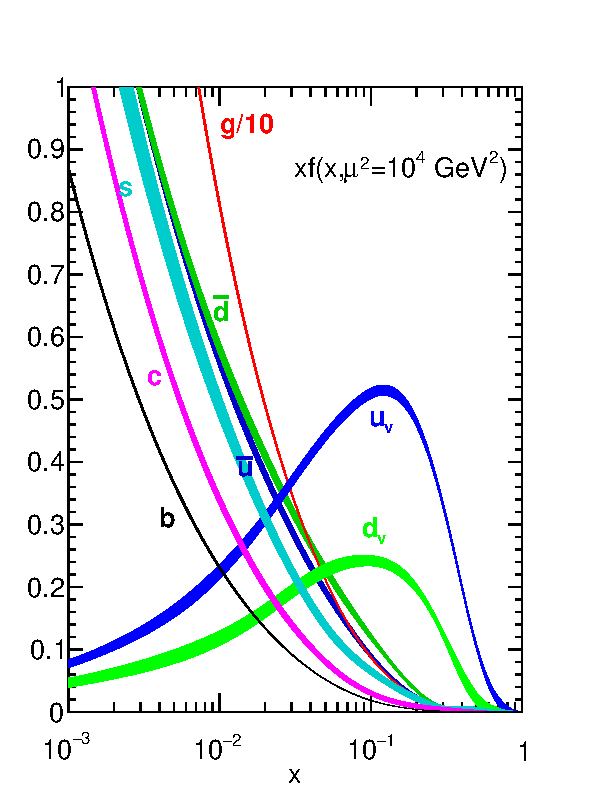
\includegraphics[scale=0.65]{Strong-Interaction/nnpdf31nnlo-1e4.pdf}
  \caption{\small Different PDFs as obtained  at NNLO level (NNPDF3.1) from Ref.~\cite{Ball:2017nwa}, evaluated
    at $\mu^2=10~{\rm GeV}^2$ (left) and $\mu^2=10^4~{\rm GeV}^2$ (right).
    \label{fig.pdf}
  }
\end{center}
\end{figure}
%%%%%%%%%%%%%%%%%%%%%%%%%%%%%%%%%%%%%%%%%%%%%%%%%%%%%%%%%%%%%%%%%%%%%%
Many of the observables that are
  studied at the LHC in most cases  depend on more than one energy scale, and thus, all order resummation   become necessary to describe the kinematic regimes in which the logarithms of ratios of these scales become large.
There are different successful approaches to calculate the resummed expressions. Another approach to the resummation is based on methods of soft-collinear effective theory (SCET) of QCD~\cite{Bauer:2000ew,Bauer:2000yr,Bauer:2001ct,Bauer:2001yt,Bauer:2008dt,Bauer:2008jx}.
In the SCET the resummation follows the concept of Collins, Soper and Sterman~\cite{Collins:1984kg} where the starting point is  the derivation of a factorisation theorem for the specific cross section and then  calculations of all logarithmic terms from  the renormalisation group evolution equation, resulting in analytic expressions for resummed cross section.  An alternative approach is based on the branching formalism\cite{Catani:1990rr,Catani:1991kz} where resummation is usually performed using the Monte-Carlo algorithm.  Both approaches have already been applied to obtain higher order resummations in the hadronic collisions
~\cite{Bozzi:2005wk,Bauer:2002nz,Banfi:2004nk,Becher:2010tm,Stewart:2010pd,Banfi:2011dx,Berger:2010xi,Jouttenus:2011wh,Becher:2012qa,Zhu:2012ts,Banfi:2012jm,Becher:2013xia,Stewart:2013faa,Procura:2014cba,Li:2016ctv,Monni:2016ktx,Bizon:2017rah}.
%%
The improvement of theoretical predictions   with increasing  accuracy of perturbative calculations    N$^k$LO  and  resummation  N$^k$LL is observed in different relevant  processes. In Fig.~\ref{NLL} we show 
 as an example   the  theoretical predictions for  the normalised  transverse-momentum  distribution  of the  Higgs  boson from  gluon fusion  at  13 TeV pp collisions,
 calculated to  different orders in perturbative QCD~\cite{Bizon:2017rah}.
  In this figure,
   the Higgs-boson transverse-momentum spectrum at N$^3$LL   is matched to fixed  NNLO   and compared to NNLL   matched to NNLO, as well as  to the pure    NNLO results.  All curves in Fig.~\ref{NLL}  are normalised to the  total  N$^3$LO cross section.

%%%%%%%%%%%%%%%%%%%%%%%%%%%%%%%%%%%%%%%%%%%%%%%%%%%%%%%%%%%%%%%%%%%%%
%\cite{Bozzi:2005wk} -\cite{Bizon:2017rah}.
%
\begin{figure}[t]
\begin{center}
%  \includegraphics[scale=0.28]{xu-31-nnlo-LHC.pdf}
  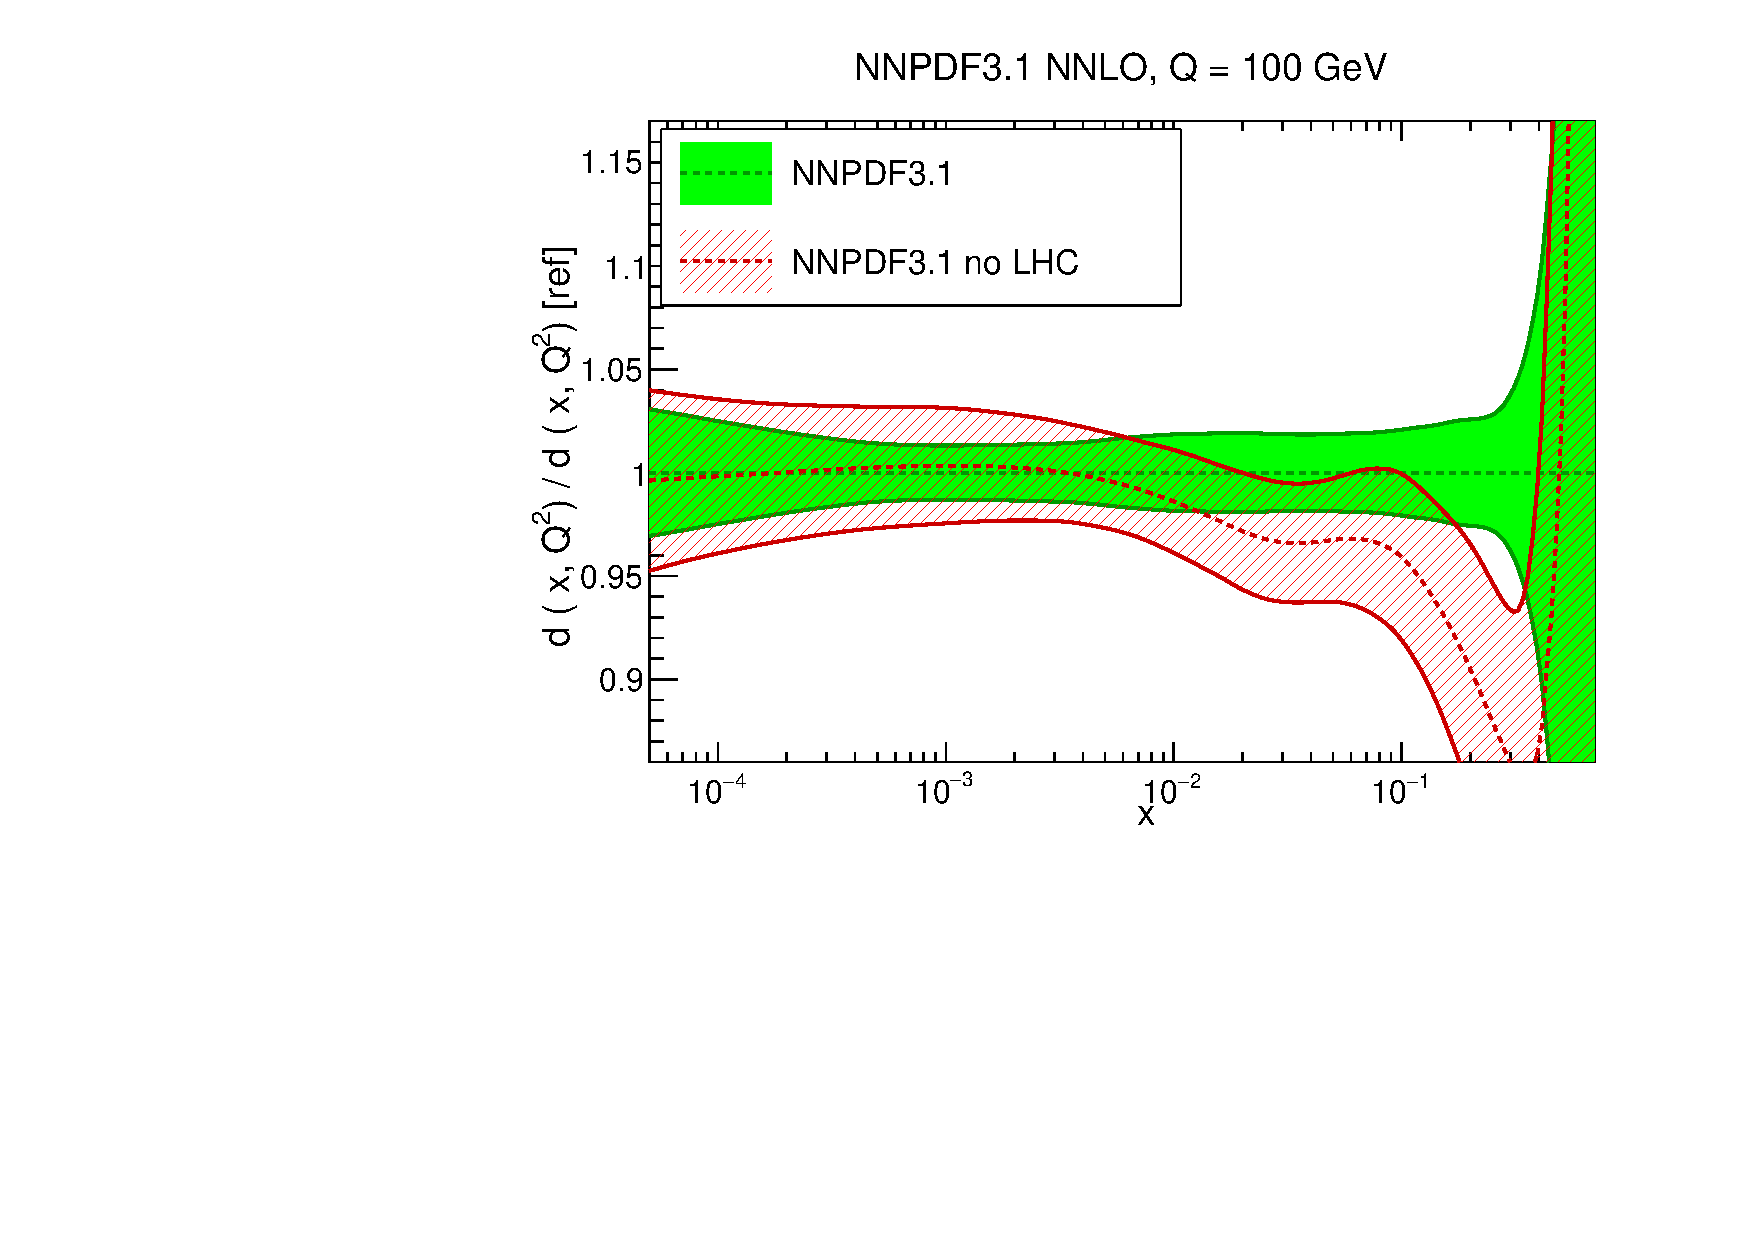
\includegraphics[scale=0.35]{Strong-Interaction/xd-31-nnlo-LHC.pdf}
  \includegraphics[scale=0.35]{Strong-Interaction/xc-31-nnlo-LHC.pdf}
%  \includegraphics[scale=0.28]{xg-31-nnlo-LHC.pdf}
  \caption{\small
The impact of the LHC data on the NNPDF3.1 NNLO PDFs  for the down and charm quarks~\cite{Ball:2017nwa}.
    %
\label{fig.impact}}
\end{center}
\end{figure}
%%%%%%%%%%%%%%%%%%%%%%%%%%%%%%%%%%%%%%%%%%%%%%%%%%%%%%%%%%%%%%%%%%%%

 The  need of improvement of theoretical predictions with increasing order of perturbative calculations    is clearly identified  in  Fig.~\ref{NLL}.
Thus, the  accurate theory calculations for collider processes are crucial to interpret the precise experimental data and to discern whether experimental measurements differ from  the SM predictions.  To match the precision of the data, theory uncertainties should be reduced to  the one  percent level for the core-  and to the few percent level for complex-processes. Furthermore, accurate theoretical predictions for BSM effects are highly desirable for  new physics searches. 
This requires a
relentless effort to improve the  understanding of QCD, by computing higher order
corrections for a larger number of processes and by refining the  theoretical and numerical  methods.
Resummed calculations are instrumental to reach an accurate description of many observables at the LHC and beyond. The understanding of regions of validity of perturbation theory, non-perturbative  and collective effects, as well as     description of very high-multiplicity final states which 
  can  provide    insights  about  the  dynamics  of  multi-particle production arising from the saturated gluon fields inside the protons,
is theoretically challenging.


A further area of active research concerns General purpose Monte Carlo event-generators. These are an essential part of the Collider QCD toolkit, being crucial for the vast majority of collider measurements and studies. Over the coming years it will be important to sustain progress on a number of fronts: (1) perturbative improvements for matching and merging (e.g. generalisation of existing approaches for parton shower + NNLO merging); (2) understanding and exploiting the relation between parton-shower algorithms and resummation to obtain higher accuracy parton showers; and (3) the further development of phenomenological models (notably those for hadronisation and the underlying event).





 \subsection{ Parton Distribution Functions}
%\\

The quest for precision at the LHC  requires
%not only   improvements  of   the accuracy of perturbative calculations but also 
a precise knowledge of the  Parton Distribution Functions  of the proton. An incomplete  knowledge of PDFs  is one of the main limitations in searches of new physics at the LHC.   At present,
PDFs cannot be  computed from first principles, although there are already
attempts to access the parton distribution functions based on LQCD simulations~\cite{Lin:2017snn}. The PDFs
have to be extracted from  the experiments, through  a careful comparison of theoretical predictions to experimental data.
Moreover, to obtain consistent predictions, it is crucial that the advancement in perturbative calculations goes together  with PDFs determination  with equal or higher  accuracy.

In recent years a new generation of PDF sets  have been developed for use at the LHC Run II, and some of  these ~\cite{Ball:2014uwa,Dulat:2015mca,Harland-Lang:2014zoa} have been combined  in the construction of the PDF4LHC15  sets which  broadly represent the present understanding of the proton structure.
%%%%%%%%%%%%%%%%%%%%%%%%%%%%%%%%%%%%%%%%%%%%%%%%%%%%%%%%%%%%%%%%%%%%
\begin{figure}[t]
\begin{center}
%  \includegraphics[scale=0.28]{xu-31-nnlo-LHC.pdf}
  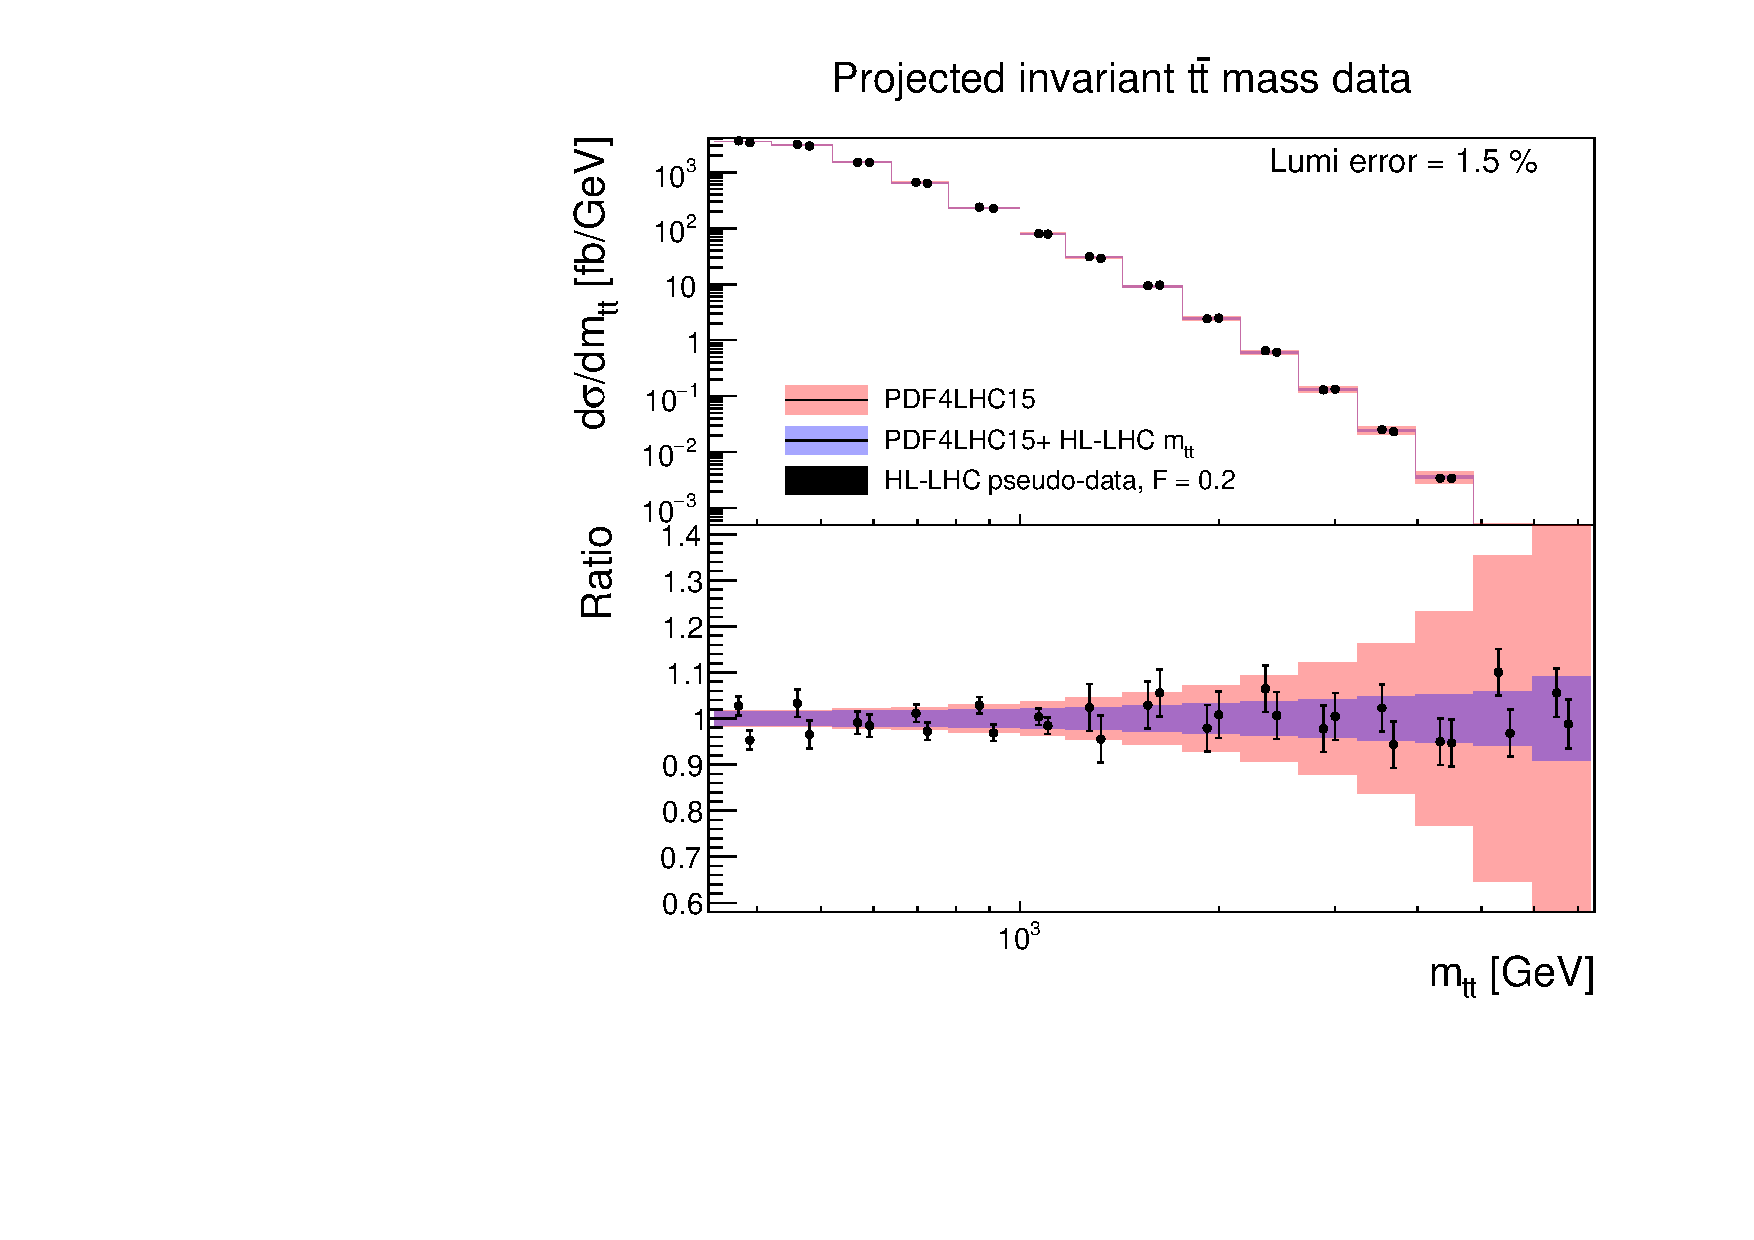
\includegraphics[scale=0.5]{Strong-Interaction/mtt_output_F_0_2_data.pdf}
%  \includegraphics[scale=0.28]{xc-31-nnlo-LHC.pdf}
%  \includegraphics[scale=0.28]{xg-31-nnlo-LHC.pdf}
  \caption{\small
Comparison between  HL$–-$LHC pseudodata and the theoretical predictions for
the $m_{t\bar t}$ distribution in top quark pair production   from Ref.~\cite{Khalek:2018mdn}. The theory calculations are shown both before (PDF4LHC15) and after  (PDF4LHC15-HL LHC) constraining PDFs  with  pseudodata  in the fit.}
\label{fig.hllhc}
\end{center}
\end{figure}
%%%%%%%%%%%%%%%%%%%%%%%%%%%%%%%%%%%%%%%%%%%%%%%%%%%%%%%%%%%%%%%%%%%%%%
Further  update  in global PDF
was  due to the progress  in  methodology  and  the available  set of new  data with
 the increasingly significant role played by LHC processes which provided stringent PDF constraints. The combination of high precision LHC data of the ATLAS, CMS and LHCb experiments   with state-of-the art NNLO theory calculations for such hadronic processes as  the transverse momentum spectrum of the $Z$ and $W$ bosons ~\cite{Boughezal:2015dva,Ridder:2015dxa}, the top-quark pair production~\cite{Czakon:2015owf,Czakon:2016dgf},  and inclusive jet production~\cite{Currie:2013dwa,Currie:2016bfm} have had  an important impact on precision PDF fits~\cite{Ball:2017nwa}. The  recent  PDF sets  NNPDF3.1 by the NNPDF Collaboration~\cite{Ball:2017nwa} are shown in   Fig.~\ref{fig.pdf}.
To illustrate the impact of the LHC  Run-1  data in the fits, Fig.~\ref{fig.impact}  compares the  NNPDF3.1 fit  with and without  LHC data at Q = 100 GeV   for the down and charm quarks~\cite{Ball:2017nwa}.  The  impact of the LHC data for $x\leq 0.005$ can be observed in this figure,  both  for  central  values  and  for  the  PDF  uncertainties.  Most PDFs are affected at the one-sigma level and in  the  case of down and charm quarks,  at up to the two-sigma level.
   Thus, it is clear that the addition of data from Run-2 and -3 and next    from the   HL-LHC,  for  which  the  precision  and  reach  will  be  greatly  increased,  should  lead  to further improvements in the determination of the proton structure. In  Fig.~\ref{fig.hllhc} we show
the comparison between the HL$–-$LHC pseudodata and the theoretical predictions on  the   $m_{t\bar t}$ distribution in top quark pair production~\cite{Khalek:2018mdn}.  There is  a clear reduction of the  PDF uncertainty    at large values of the invariant mass.

 Currently, PDF uncertainties account mostly for the propagated statistical and systematic  errors  on  the  measurements  used  in  their  determination. Clearly, the missing higher order uncertainties  from the truncation of the QCD perturbative expansion also affect predictions for the various processes that enter the PDF determination. The    PDF extraction that systematically accounts for these effects  in  QCD calculations   and assesses  their impact on the  uncertainties of the resulting PDFs, has been recently considered~\cite{AbdulKhalek:2019bux}.
%

%%%%%%%%%%%%%%%%%%%%%%%%%%%%%%%%%%%%%%%%%%%
%%%%%%%%%%%%%%%%%%%%%%%%%%%%%%%%%%%%%%%%%%%
The ultimate method to determine the parton structure of the proton is with high precision, high energy measurements in electron-proton
scattering. The LHeC and FCC-eh provide a complete resolution of PDFs, of both protons and ions,  as has been described recently in \cite{Ides159,Klein:2018rhq}. High $x$, which is crucial for searches at $pp$ colliders, is clarified, both the valence quark, small but important sea and gluon contributions, due to the high luminosity and large $Q^2$ lever arm. At medium $x$ sub-percent precision for N$^3$LO PDFs is reached due to the unique measurement techniques of electrons, neutrinos and the hadronic final state. Flavour is completely resolved owing i) to the high energy enabling to access charged current cross sections for many orders of magnitude in $x$ and
ii) to the direct measurements of strange, charm and beauty densities. Finally, the long standing quest of a possible saturation of the gluon density at small $x$ and the existence of non-linear evolution terms, rendering the DGLAP formalism obsolete, will be definitely solved at the LHeC. All of this maybe illustrated, in a yet simplified manner, with the ultimate accuracy one would achieve with LHeC (and FCC-eh in an extended range) for the various parton-parton luminosities, see
Fig.~\ref{figlumisep}.
%%%%%%%%%%%%%%%%%%%%%%%%%%%555
\begin{figure}[t]
\centering
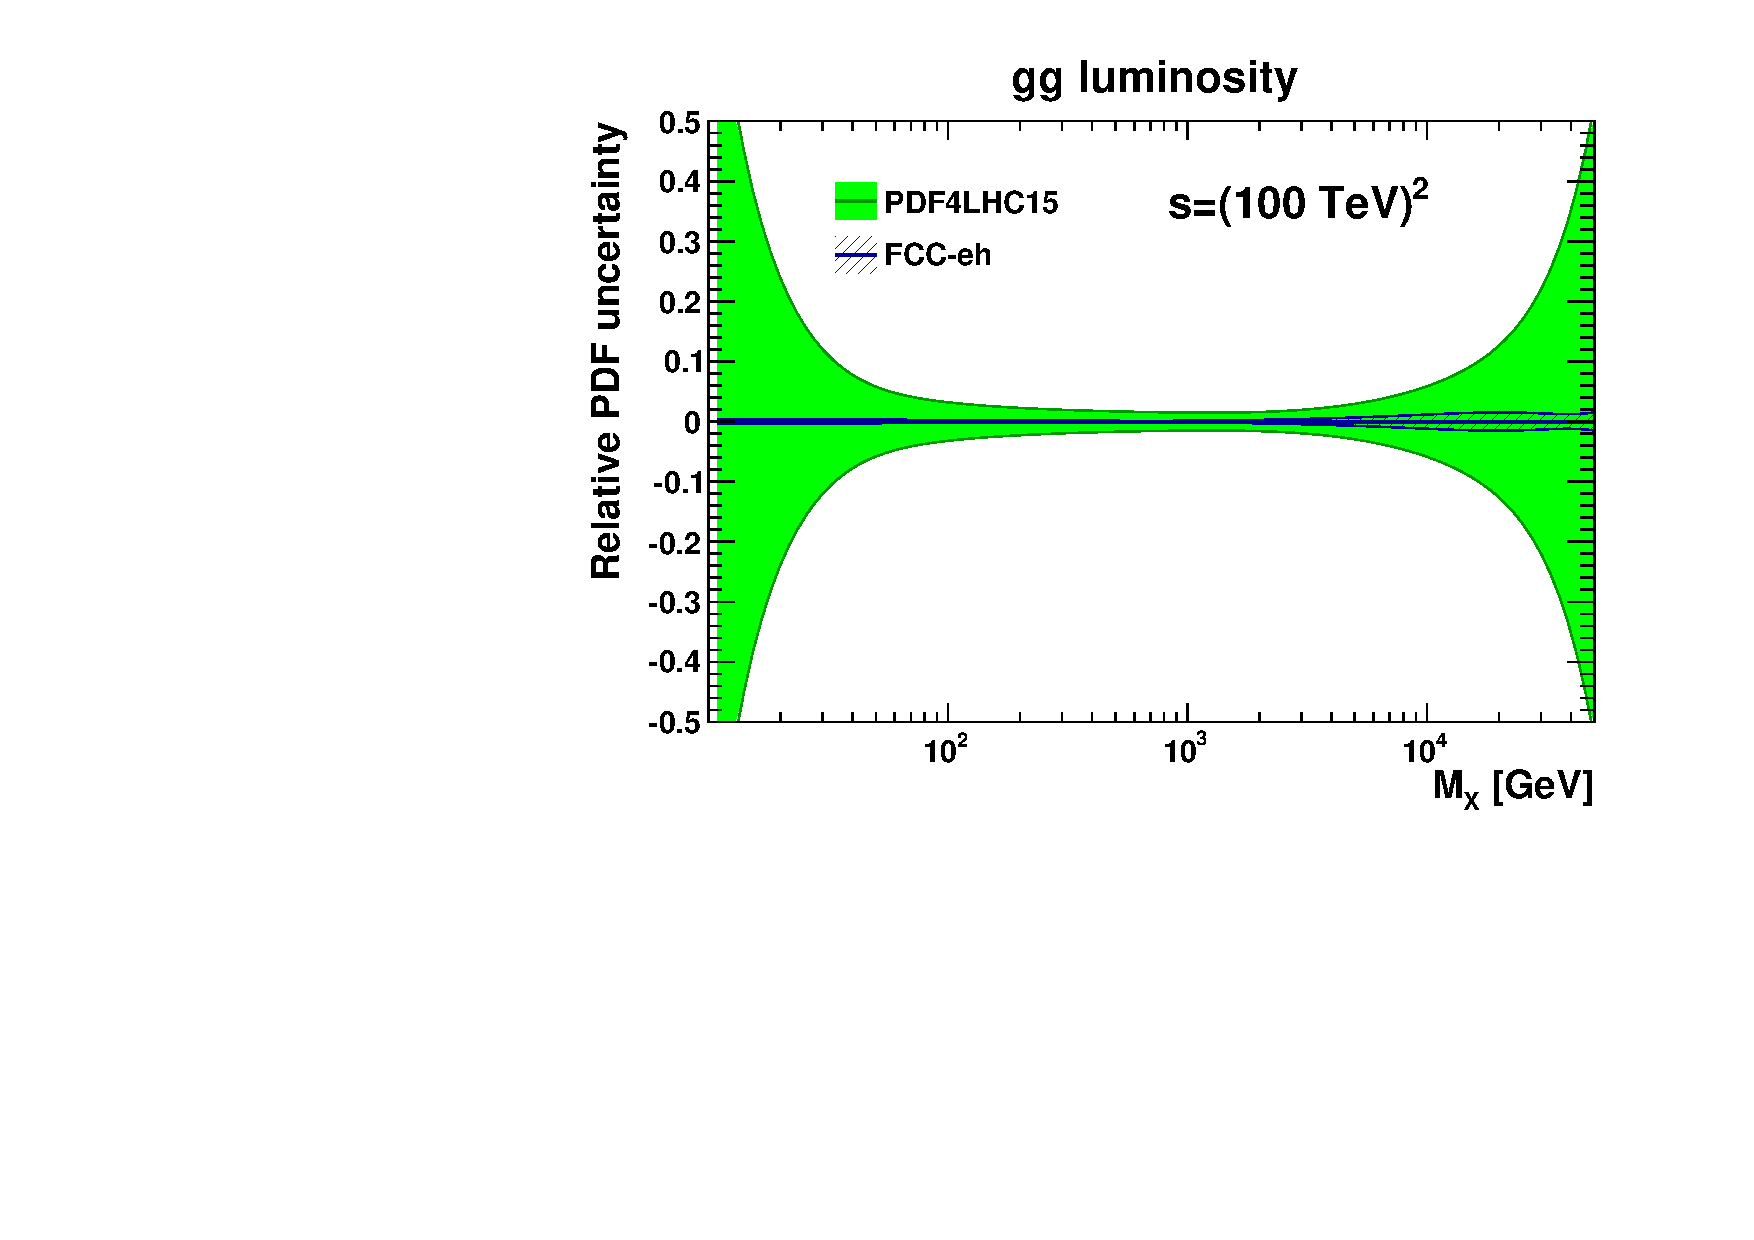
\includegraphics[width=0.5\textwidth]{Strong-Interaction/frac_gg_vs_mx_log.pdf}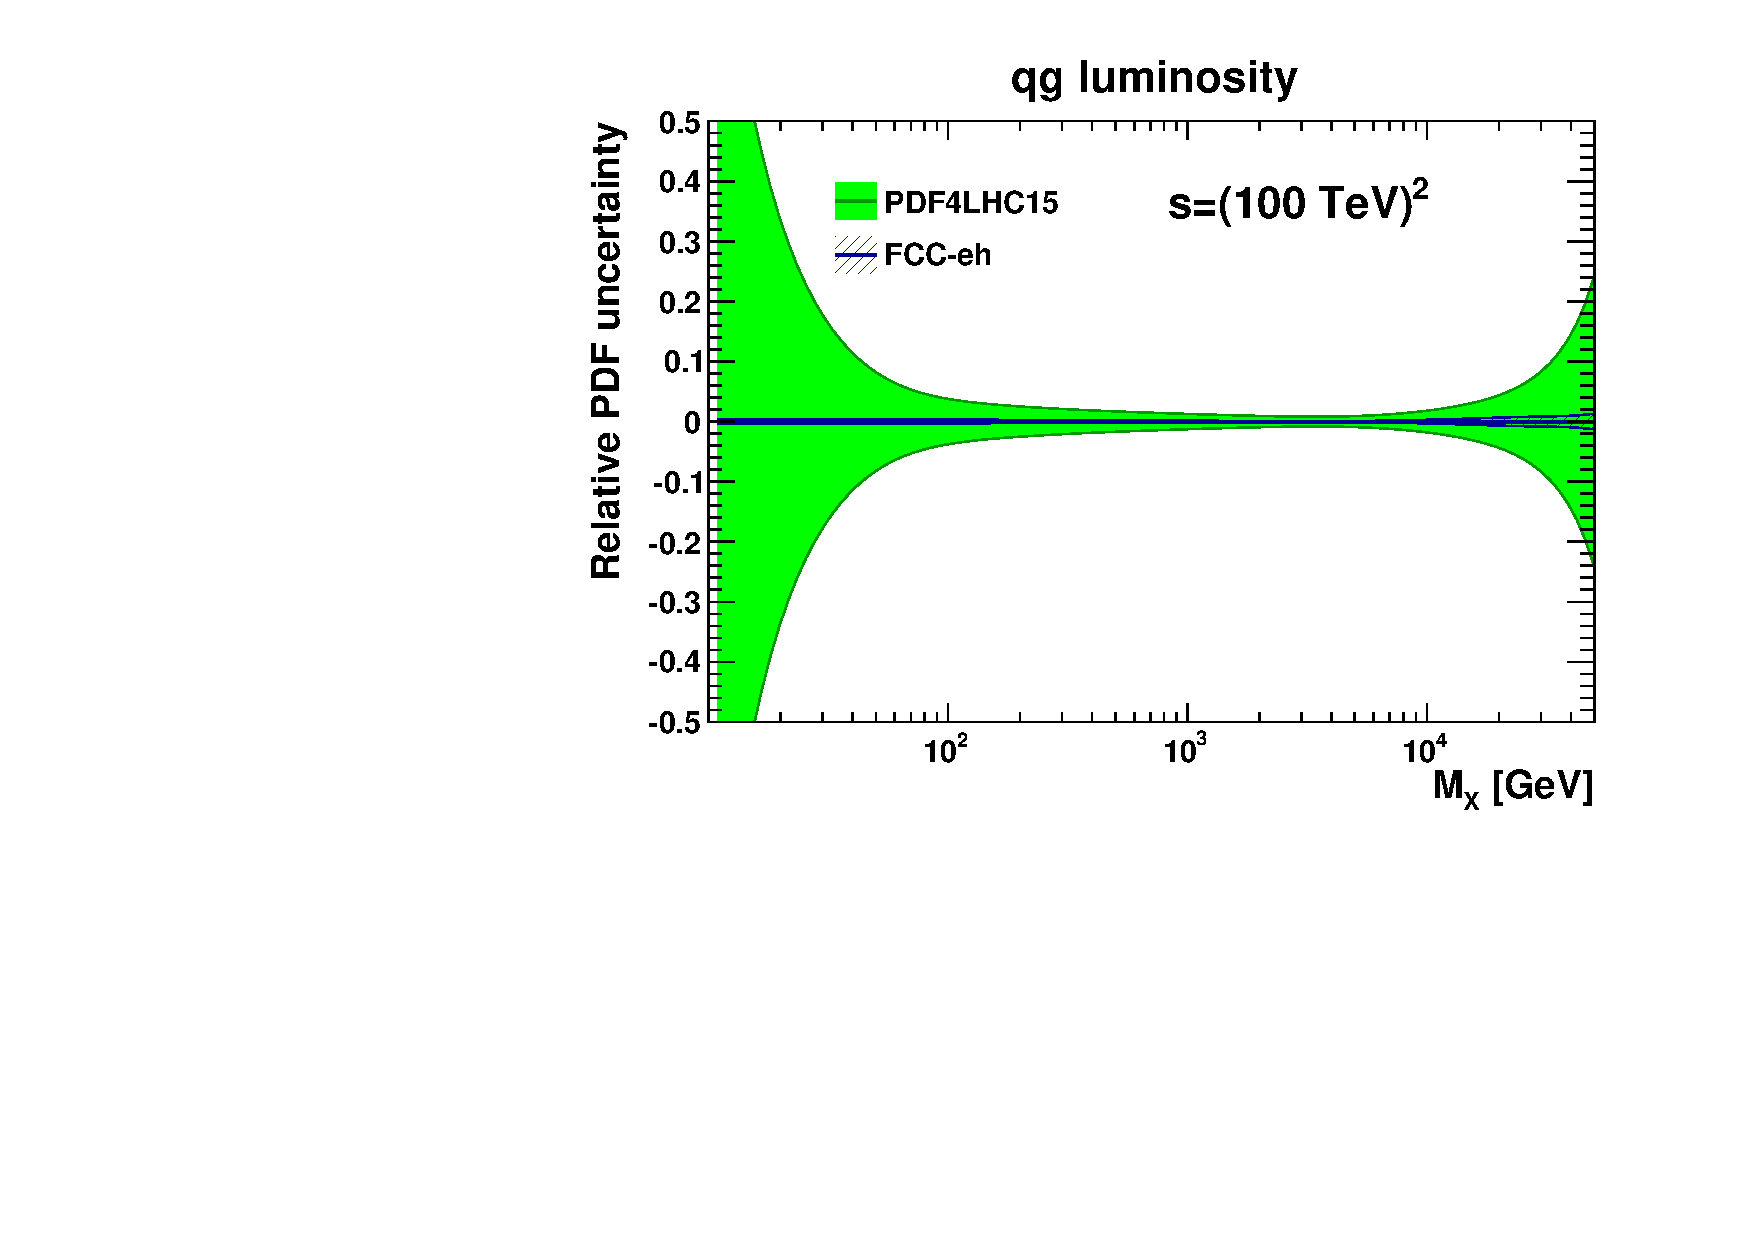
\includegraphics[width=0.5\textwidth]{Strong-Interaction/frac_gq_vs_mx_log.pdf}\\
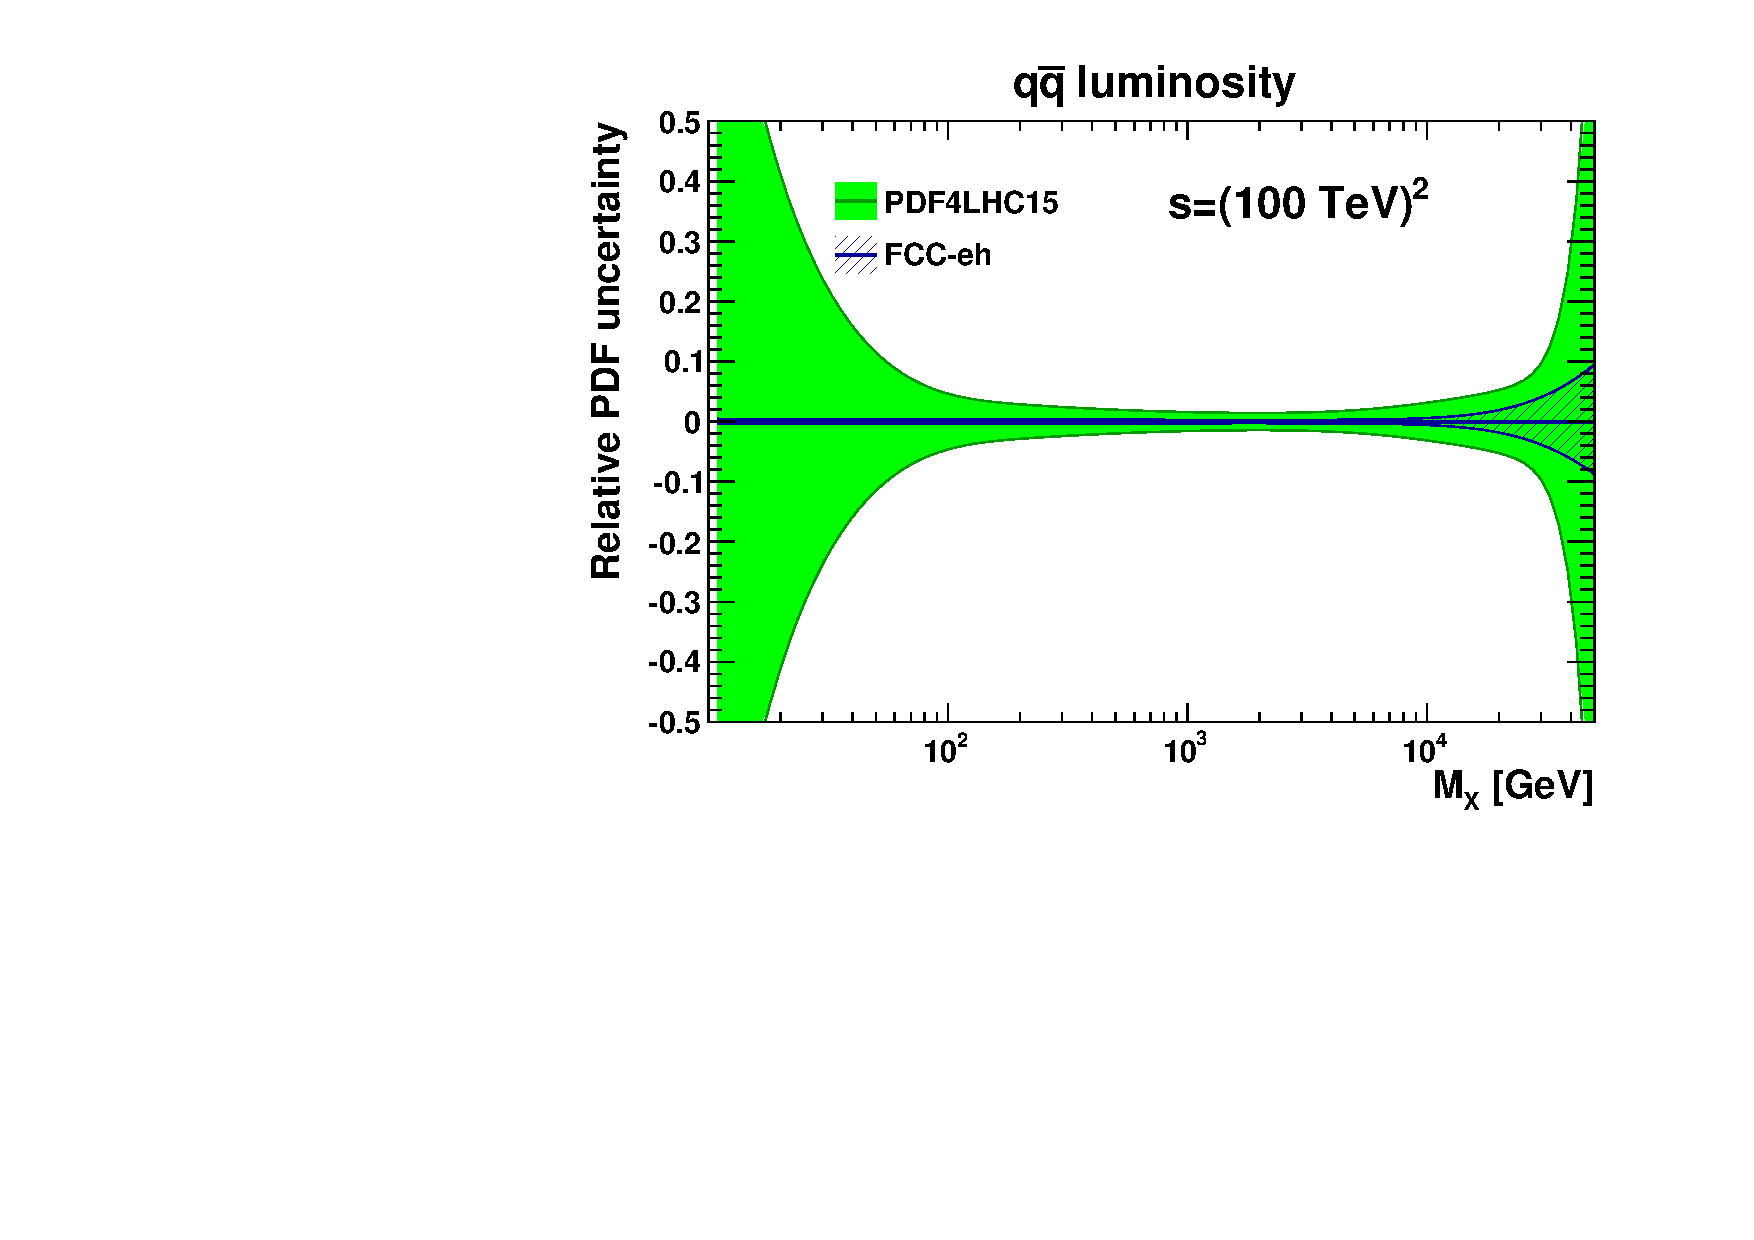
\includegraphics[width=0.5\textwidth]{Strong-Interaction/frac_qqbar_vs_mx_log.pdf}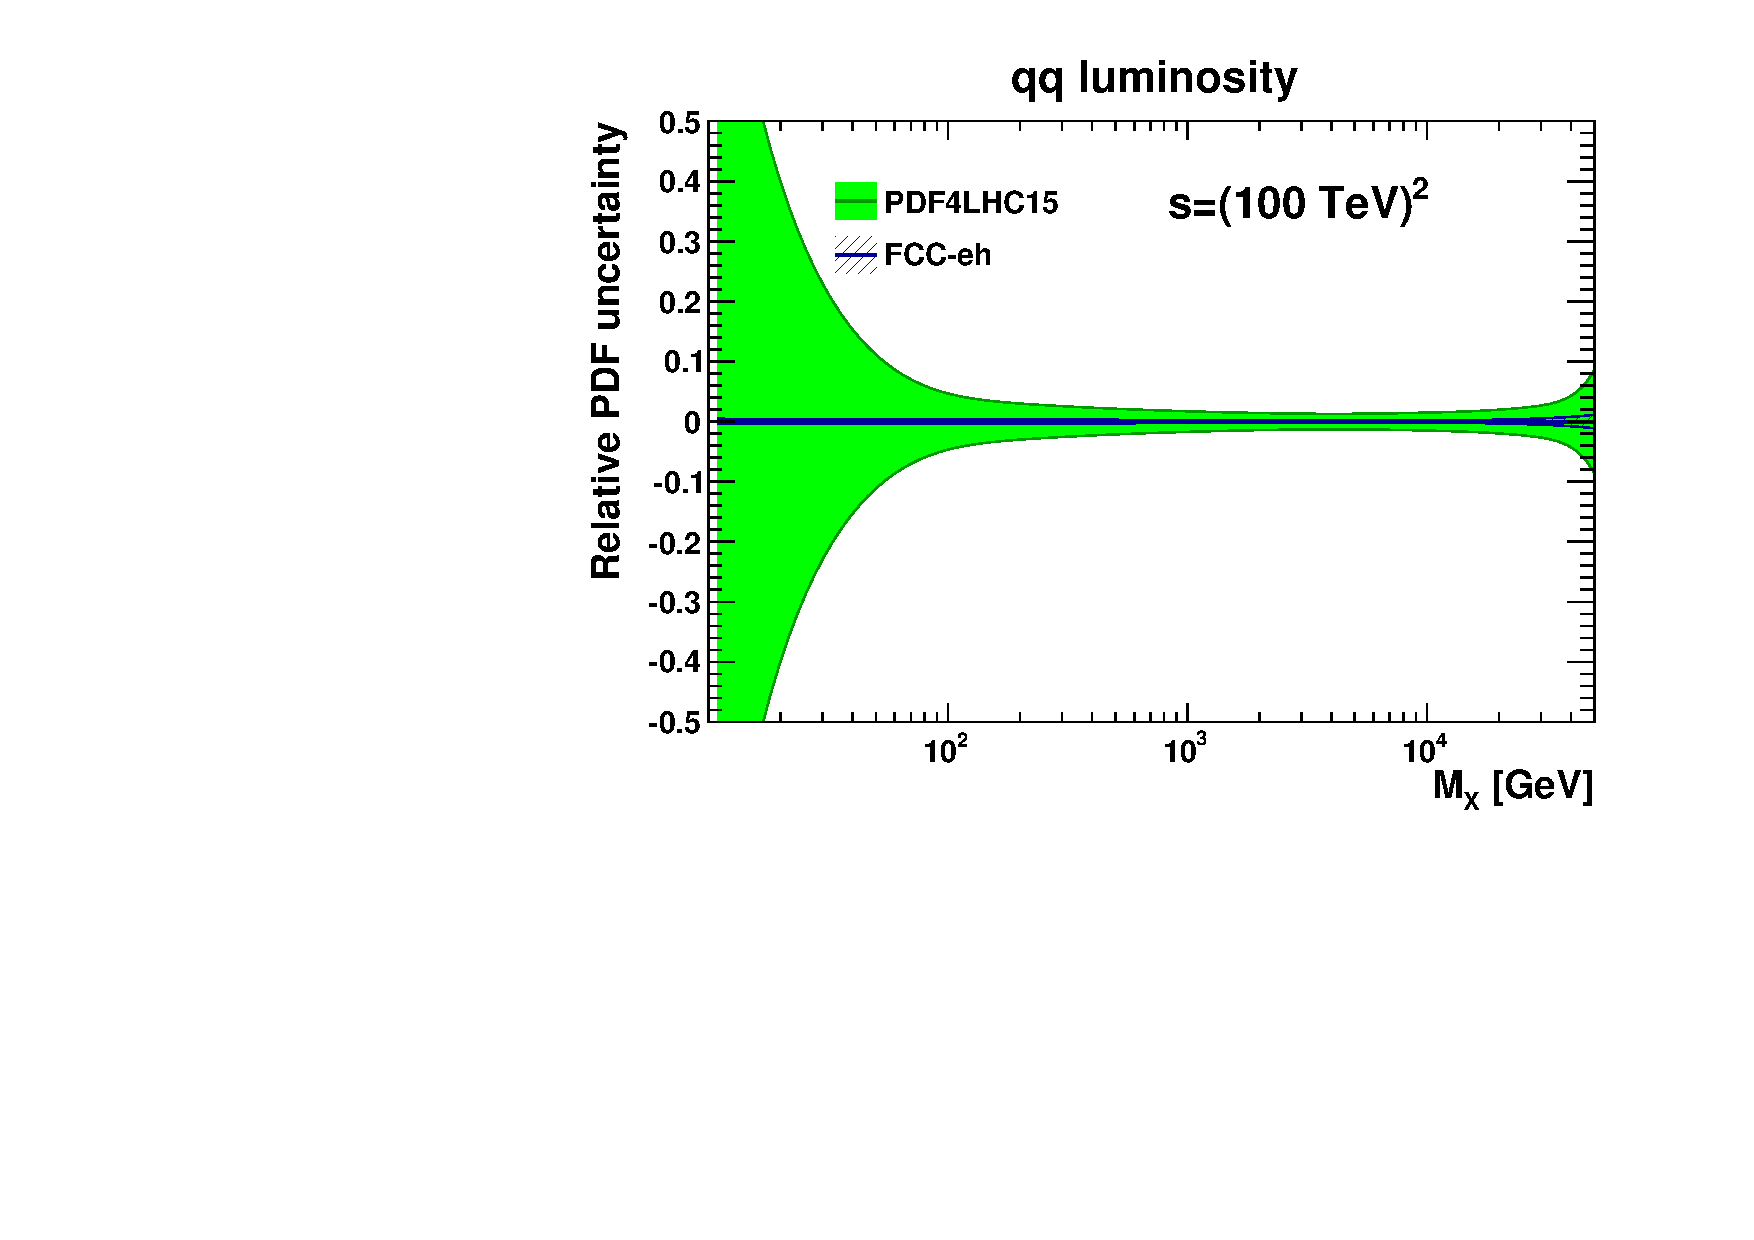
\includegraphics[width=0.5\textwidth]{Strong-Interaction/frac_qq_vs_mx_log.pdf}
\caption{{Relative PDF uncertainties on parton-parton luminosities from
the PDF4LHC15
and FCC-eh PDF sets, as a function of the mass of the produced heavy
object, $M_X$,
at $\sqrt{s} = 100$ TeV. Shown are the gluon-gluon (top left),
quark-gluon (top right), quark-antiquark (bottom left) and quark-quark
(bottom right) luminosities. The LHeC expectation is very similar but
misses one order of magnitude towards low $x$.}}
\label{figlumisep}
\end{figure}

 The full programme can also be pursued in electron-ion scattering which will represent  a genuine contribution to our deep 
understanding of nuclear substructure. This programme
extends the search range in $pp$ towards higher masses and enables
precision electroweak and Higgs physics at the LHC/FCC-hh. Of principal
importance is to disentangle predictions and effects from QCD/PDFs from
possible new physics. DIS and LHC would provide two independent
configurations for achieving this while $pp$ alone could   run into the conceptual problem of possibly taking new phenomena as (large or small
$x$) PDF or QCD effects. In nuclei one needs to disentangle nuclear
environment (shadowing) from non-linear (BFKL) effects. All this
requires very high precision, very high energy, large luminosity $ep$ and
$eA$ collision data taken while LHC is operational (and later
synchronously through FCC-hh and FCC-eh operation). 

%%%%%%%%%%%%%%%%%%%%%%%%%%%%%%%%%%%%%%%%%%%%%
%%%%%%%%%%%%%%%%%%%%%%%%%%%%%%%%%%%%%%%%%%%%
Given the high precision expected for HL-LHC data, it will be crucial to include all sources of experimental, methodological, and theoretical uncertainties associated with PDFs in order to ensure robust predictions. In particular,
the impact of theoretical uncertainties due to the missing higher-order corrections in theoretical calculations,  the fits with high-energy and threshold logarithms resummed and    the contribution of  electroweak corrections  should    be analyzed and included in the determination of  global PDFs in the foreseeable future. Furthermore, as already pointed out in in Sect.~\ref{section_low},  a  precision physics programme at future hadron colliders requires    a more detailed  description  of  
the partonic substructure of hadrons   as encoded  e.g. in GPDs or  TMDs. Theoretically challenging is also the phenomenon  of  saturation of partonic densities  at small enough values of  the  fraction  of  momentum $x$, which has  developed into a complete and coherent formalism of the Colour Glass Condensate ~\cite{Iancu:2002xk,Petreska:2018cbf,Altinoluk:2019fui}. Furthermore,  a reliable determination     of the parton distribution functions of nucleons bound within nuclei (nPDFs),  is particulary relevant for precision phenomenology and   fundamental understanding of the strong interactions in the nuclear environment~\cite{Kusina:2017gkz,AbdulKhalek:2019mzd}.




%%%%%%%%%%%%%%%%%%%%%%%%%%%%%%%%%%%%%%%%%%%%%%%%%%%%%%%%%%%%%%%%%%%
\subsection{ Numerical Lattice  QCD}


Many of the SM  predictions require the knowledge  of  parameters and observables  which encode nonperturbative QCD effects.  They can only be calculated from first principles  by using numerical lattice QCD~\cite{Aoki,Bazavov:2019lgz,Cirigliano:2019jig}.

Over the past years, an increased computing power, together with   the development of better algorithms and  analytical frontiers  techniques have enabled realistic LQCD predictions   with controlled errors. LQCD allows for a  precise  determination of a wide range of hadronic observables, including the hadron masses and  decay constants, form-factors and mixing parameters characterising weak-decay amplitudes,  parton distribution functions, as well as key SM parameters such as quark masses and the QCD coupling~\cite{Aoki}.
LQCD    provides   the most precise determination of the strong coupling constant~\cite{Patrignani:2016xqp,Aoki:2016frl},  and the high accuracy    results for  the  $D$, $D_s$, $B$, and $B_s$ heavy flavour meson decay constants  with sub per-cent precision~\cite{Bazavov:2017lyh}. Similar precision  has been reached in the determination of the  light ($u,d,s$) and heavy flavour ($c,b$) quark  masses~\cite{Bazavov:2018omf}.
 Further  LQCD results on  $B\to \pi$ and  $B\to K$ semileptonic form factors, neutral kaon mixing  and neutral $B_d$- and $B_s$-meson  mixing~\cite{Dowdall:2019bea}  led to significant improvements in the determination of the Cabibbo-Kobayashi-Maskawa   quark-mixing matrix elements and the global unitarity-triangle fit.
The  unprecedented  accuracy  of  lattice calculations  and  state-of-the-art  techniques    allowed one to extract the nucleons  electromagnetic and axial  form  factors and their electromagnetic radii and the magnetic  moments~\cite{Alexandrou:2018sjm,Alexandrou:2018lvq,Djukanovic:2019jtp}.
Inspired by the LHCb discovery of  a  new  narrow  charmonium  state,  the $X$(3842)~\cite{Aaij:2019evc}, LQCD presented  calculations   of   charmonium states  near the open-charm threshold by   means of  the  L\"uscher  formalism, and found  the charmonium resonance with $J^{PC}=3^{--}$ and the mass consistent with the $X$(3842)~\cite{Aaij:2019evc}.  The  recent  LQCD  calculations  of exotic states in  QCD,  also predicted    the existence of a  doubly-bottom $(\bar b\bar b ud)$ tetraquark bound state that is stable under the strong and electromagnetic interactions~\cite{Piemonte:2019cbi}.



In the  ongoing search for new physics beyond the Standard Model,  LQCD   provides results  for  the  nucleon  scalar and tensor charges~\cite{Aoki,Alexandrou:2017qyt}, as well as demonstrates   the feasibility of  computing the amplitude of rare kaon decay $K^+\to \pi^+ \nu\bar\nu$~\cite{Bai:2018hqu}, the process   which is experimentally  studied  by   the NA62 experiment at the CERN SPS. LQCD has also addressed the issue of the  CP violation in the QCD sector.   Interesting results are obtained  in recent LQCD calculations  for  the  electric dipole moment (EDM)  of the nucleon induced by the QCD $\theta$ term~\cite{Dragos:2019oxn}. The  results  indicate  that the EDM of the nucleon stays finite in  a continuum and the chiral limit.  This result together with the experimental bound on    the neutron EDM provide the  upper limit     for  the value of QCD $\theta$ term.   
Enormous progress has also been achieved in ab-initio  lattice  calculation of  the strong interaction contribution $a_\mu^{\rm had}$  to the anomalous magnetic moment of the muon $g-2$~\cite{Meyer:2018til,Westin:2019tgc}.  LQCD
provides  results on   the   hadronic  vacuum polarisation (HVP) and hadronic light-by-light (HLbL) scattering contributions to $a_\mu^{\rm had}$. While the  error of current LQCD estimates of the HVP reached  the few-percent level, the 
 uncertainty in the  determination of a HLbL is  at the $(10-15)\%$-level. The goal for the future LQCD calculations is  the sub-percent precision  of a HVP contribution  which is needed to reduce the SM uncertainties  on the value of  $g-2$ to possibly  identify  new physics  by   comparison to the  experimental data.

LQCD methods are also very successful  in describing  thermodynamic   properties
and structures of the strongly interacting matter under extreme conditions of high temperature $T$  and  density $\rho$~\cite{Bazavov:2019lgz,Andronic:2017pug,Soltz:2015ula,Ding:2015ona,Ratti:2018ksb}.  Such a QCD matter  is produced in ultra-relativistic $AA$ collisions, $pA$ and possibly  even   in the high energy and high multiplicity events in $pp$ collisions~\cite{Citron:2018lsq}.  LQCD   describes   the phase structure of  strongly interacting matter,   nature of QCD  phase transition and the equation of state. Large scale computing has allowed one to quantify  the value and the shifts of the chiral critical temperature from the  chiral limit  to the physical point. The shift of the pseudocritical temperature with finite chemical potential  $\mu_B$ has also been  recently established up to $(\mu/T)^4$ order~\cite{Bazavov:2018mes}  (see Fig.~\ref{fig:Tmub}). LQCD provides  calculation of  correlations, diffusion and transport properties  in  a quark-gluon plasma and  fluctuation observables~\cite{Soltz:2015ula,Friman:2011pf,Karsch:2010ck}  that are directly linked to experimental data. LQCD predictions are essential  inputs to hydrodynamic-   and transport-model description of experimental data   in $AA$ and  $pA$   collisions~\cite{Citron:2018lsq}.

Continued efforts  and support in developing new theoretical methods and better algorithms are needed in  LQCD  to reach the  anticipated progress and  precision   of  SM  predictions  and to  sharpen  opportunity for new physics  discovery.  In high density QCD, more detailed studies close to the chiral limit and on large lattices are needed to reach  definitive  conclusions  on  the  role  of the  $U_A(1)$ symmetry  breaking   and the order of the chiral phase transition. To  have  impact  on  the experiments in  future,  LQCD  calculations  of  electromagnetic  probes, fluctuation observables, spectral functions   and transport properties   of  QGP  need  to be carried out with high statistic on large lattices and with physical dynamical quarks. The problem of finite chemical potential in LQCD calculations needs a further attention to develop an efficient  formalism that allows for lattice simulations
with a complex action.
%%%%%%%%%%%%%%%%%%%%%%%%%%%%%%%%%%%%%%%%%%%%%%%%%%%%%%%%%%%%%%%%%%%
%%%%%%%%%%%%%%%%%%%%%%%%%%%%%%%%%%%%%%%%%%%%%%%%%%%%%%%%%%%%%%%%%%%

\subsection{The strong coupling constant $\alpha_s$}
%\JDH{0.5p}}

%The role of this measurement in the context of the exploration of particle physics and the search for new physics at high energies. The roles of future $\Pep\Pem$, $ep$ and $pp$ programmes and the opportunities, challenges and requirements for theory and Lattice QCD efforts.

The strong coupling is the least known fundamental coupling in the Standard Model. This becomes a hinderance for precision measurements, such as of the Higgs production cross sections and couplings, and it impacts the uncertainty budget in predictions of electroweak vacuum stability and grand unification theories approaching the Planck scale.
% and it prevents precise tests for grand unification theories at the Planck scale.
Currently, the LQCD results are more precise than the values directly derived from experiment as summarised recently in refs.~\cite{Bethke:2017uli,dEnterria:2019its} and shown in Tab.~\ref{tabl}. %~\cite{Patrignani:2016xqp}.

%
% may need to be replaced by 2018 if such a table was to be included
%
\begin{table}[h]
\caption{
%Mean values of the strong coupling constant $\alpha_s(M_Z^2)$, to NNLO and for $5$ active flavours, taken from PDG2018.
World-average values of the strong coupling constant at the $Z$ mass,
$\alpha_s(m_Z)$, at NNLO accuracy for 5 active
flavours~\cite{Tanabashi:2018oca}.
}
\begin{center}
\begin{tabular}{|c|c|}
\hline
Method & $\alpha_s(M_Z^2)$ \\
\hline
Lattice QCD & $ 0.1188 \pm 0.0011$ \\
$\tau$-decays & $ 0.1192 \pm 0.0018$ \\
DIS & $ 0.1156 \pm 0.0021$ \\
Hadron Collider & $ 0.1151 \pm 0.0028$ \\
Electroweak Fits & $ 0.1196 \pm 0.0030$ \\
$e^+e^-$  & $ 0.1169 \pm 0.0034$ \\
\hline
\end{tabular}
\label{tabl}
\end{center}
\end{table}

New measurements of $\alpha_s$ at the level of
per mille accuracy are mandatory and could be achieved with FCC-ee from the ratio of the hadronic-to-leptonic
width at the Z-pole and with LHeC/FCC-eh from the scaling violations of
the structure functions.
Both demand a new level of theoretical support to
develop theory one order of perturbation further. Both also require
extreme experimental care and additional cross
checks, e.g.\ from the $W$ in $e^+e^-$ and from jets in $e^+e^-$ and DIS,
respectively, to assure a maximum of confidence and enhanced precision.
The realisation of this complementary programme would be a major
milestone in the development of QCD and in the  reduction of important parametric uncertainties today in key SM and BSM theoretical calculations.
% in our understanding of the details of a possible grand unification scheme and, thus, of nature.
It would also be a
major triumph of experimental physics and its intimate collaboration with theory. The challenge of LQCD at this high level of accuracy will surely lead to new insight into the details~\cite{Aoki:2016frl} of
LQCD calculations as well.



\subsection{The low energy precision QCD}
%puzzle 
%\JDH{1p}}

%\begin{itemize}
%\item The proton radius puzzle (MUSE, COMPASS, several experiments, %theoretical requirements)
%\item Hadronic vacuum polarisation (MUoNe)
%\item Chiral symmetry breaking (DIRAC)
%\item Particle spectra (NA61/SHINE, COMPASS, ...)
%\item Nuclear precision with HIE-ISOLDE and the EPIC upgrade
%\end{itemize}
%\JDH{editor: 
%Klaus Kirch
% will provide text later this month}
 
 Many aspects of QCD   are important for experiments at low energies and, vice versa, various experiments at low energies yield precision QCD benchmarks~\cite{Alemany:2019vsk,Dainese:2019xrz}.

The strong CP problem~\cite{Cheng:1987gp,Pospelov:2005pr}, i.e.\ the extreme smallness of the  {\it $\theta$-term} in the QCD Lagrangian, is evident from the non-observation of permanent hadronic electric dipole moments (EDM), in particular of the neutron and of $^{199}$Hg. Considerable international efforts aim to improve the experimental sensitivity to permanent EDM of the neutron, of heavy nuclei and recently also of the deuteron, the proton and heavier baryons ~\cite{Engel:2013lsa,Semertzidis:2003iq,Afach:2015sja,Lenisa:2017okq,Chupp:2017rkp}. The most sensitive and straightforward to interpret is the neutron EDM. Experimental sensitivities should improve by two orders of magnitude to a few $10^{-28}$e.cm in the next decade. Further improvements will require R\&D into new experimental concepts to overcome statistical and systematics limitations. Similarly, the EDM of the proton can be searched for with a dedicated storage ring experiment, not statistically limited before $10^{-29}$e.cm. R\&D, precursor experiments as, e.g.\ at COSY, and prototyping can pave the way to understand and tackle the corresponding systematic issues~\cite{Lenisa:2017okq}.



Besides EDM, several finite electromagnetic form factors of the nucleons provide benchmarks for low energy QCD studies:

-          Magnetic moments of proton, antiproton and neutron are measurable at much higher precision~\cite{Mooser:2014vla,Smorra:2018syp,Smorra:2016vxa,Afach:2014fha} than calculated by theory. Nevertheless, they are important for metrological reasons and strong tests of CPT and other fundamental symmetries. The AD and Elena at CERN are essential facilities as are the neutron EDM experiments, in Europe at PSI and at ILL.

-          The proton rms charge radius continues to puzzle with discrepant results from muonic hydrogen spectroscopy at PSI, ordinary hydrogen spectroscopy and e-p scattering results~\cite{Antognini:2015moa,Pohl:2010zza,Antognini:2005fe,Bernauer:2010wm,Antognini:1900ns}. Considerable theoretical and experimental efforts, notably also $\mu$-p scattering with MUSE at PSI and potentially COMPASS$^{++}$ at CERN~\cite{Gilman:2013eiv,Denisov:2018unj}, have emerged aiming at resolving the puzzle.  Eventually LQCD calculations will contribute to corroborating the {\it true} value. The proton Zemach radius and the magnetic radius are targets of next generation muonic hydrogen experiments measuring the ground state hyperfine splitting. Experiments are planned for PSI, Riken-RAL, and J-PARC.

-          The nucleon axial form factor $g_A$ at lowest momentum transfer is determined by measurements of neutron decay correlations, in particular at ILL~\cite{Markisch:2018ndu}. An order of magnitude improvements can be envisaged with a new generation of experiments, in particular at a new fundamental physics beamline at the ESS.

-         The nucleon axial radius can be determined by muon capture on the proton~\cite{Hill:2017wgb} yielding complementary information to neutrino scattering and potentially crucial input to long baseline neutrino experiments.

QCD input is also essential in order to allow for comparisons between high precision experiments and precision SM calculations. The anomalous magnetic moment $(g-2)$ of the muon is an exquisite example and substantial theoretical and experimental efforts are presently underway in order to improve the experimental sensitivity and the accuracy of the QCD corrections. The MUonE experiment e.g.  aims at determining the leading order hadronic contribution to the muon $g-2$ by measuring the hadronic part of the photon vacuum polarisation in the spacelike region. 

The  experimental studies of  strong force and  the structure and dynamics of atomic nuclei is a vital part of strong interaction physics.
The Di-meson Relativistic Atom Complex (DIRAC)  aims to check
low-energy QCD predictions using double-exotic $\pi\pi$ and $\pi K$ atoms 
%the decay of unstable {\it pionium atoms}
to  gain a deeper insight into the quantum theory of the strong force \cite{Adeva:2018fwr,DIRAC:2016rpv}.
%Pionium  are produced using a beam from CERN Proton Synchrotron accelerator  and their  lifetime is being measured to a level of accuracy never achieved before.
The CERN ISOLDE facility  produces radioactive isotopes for studies of the structure of atomic nuclei and a variety of other purposes including medical and astrophysical applications. The phase 2 of its HIE-ISOLDE upgrade has reached completion which 
 allow ISOLDE to accelerate radioactive beams to energies up to 10 MeV per nucleon  to study a variety of nuclear reactions with radioactive isotopes, opening up new possibilities for nuclear-structure research. The {\it intensity} upgrade is foreseen for Phase 3, and will allow ISOLDE to remain at the forefront of nuclear and astrophysics research for  another decade. 



%%%%%%%%%%%%%%
\section{QCD and other disciplines}
%\JDH{1p, each subsection around 8 lines}} \JDH{editor: Jorgen}\\

%\textbf{QCD and particle physics:} The essential need for QCD studies to feed into other parts of particle physics. Include neutrino physics. \JDH{this line might be skipped}

%\textbf{QCD, technology and applications:} The need to connect to instrumentation, computing and software, machine learning, accelerators (e.g. ERL), electronics, ...

The LHeC and FCC-eh are the highest energy, highest electron current applications of energy recovery linac (ERL) technology. In itself, ERL entails major technology innovations, most obviously on high quality, superconducting cavities such as those required for the FCC-ee. 
%Unlike the ILC, an ERL is not focussed on maximum gradients but high $Q_0 \geq 10^{10}$. 
%ERL is a major stimulus for accelerator technology development for progress in SCRF which feeds back to other collider applications, such as FCC-ee. 
ERL reaches efficiencies in excess of 90\% reducing the required power, as for LHeC's 60 GeV electrons, from a GW to below 100 MW wall plug. By decelerating the beam after the interaction, the power is taken to supply the accelerating part of the ERL while the beam energy is eventually reduced to the injection energy. 
The dump of ${\cal O}(500 {\rm MeV})$  is environment friendly, in contrast to proton or electron high energy, radioactive beam dumps. 
%By operating synchronously to the HL-LHC, the LHeC makes maximum use of an existing, operating facility.
In the context of the PERLE facility at Orsay (submission ID147), the first 802 MHz prototype was built for both LHeC and FCC-ee.
%The ERL development is accompanied by lower energy (500 MeV to 1 GeV) ERL facilities, with PERLE at Orsay~\cite{ID147} as prime example for it uses the same 802 MHz frequency and the same 3-turn configuration. 
These facilities have major technical applications such as for lithography, through their laser application, or material tomography and photofission, through the intense (1000 times more intense than ELI), mono-energetic photon beams, generated by laser backscattering. Therefore, at a small fraction of the ELI cost, a new facility (or facilities) may be established that also open new avenues to photonuclear and particle physics. This is a rare example of a direct synergy between energy frontier particle and low energy nuclear and applied physics.

The low radiation and zero pile-up environment of ep colliders, combined with the demand for very high quality vertex tagging makes detectors at these facilities a most suited application for an HV CMOS silicon vertex detector, of low material and high integration level.

Laser spectroscopy of light muonic atoms has been established as a game changer in the determination of nucleon/nuclear charge radii. For these, and for the determination of Zemach radii and other spectroscopy goals in those exotic systems, the development of high power, pulsed lasers, stochastically triggerable with low latency is key.

The development of higher intensity, higher quality, low-momentum muon beams of both polarities is an essential part to further improve the measurements of the muon anomalous magnetic moment, the proton radii, and the nucleon axial radius.

%%%%%%%%%%%%%%%%%
\subsection{QCD and astroparticle physics}
The production, propagation, and detection of the most energetic particles produced in the Universe, in yet unravelled sources, relies heavily on our understanding of QCD at high energies. For both charged cosmic rays (CRs) and neutrinos, cross sections linked to QCD processes in the non-perturbative and perturbative regimes are still the largest source of theoretical uncertainty. Dedicated measurements at FCC-pp, FCC-ep, and fixed-target-LHC, in particular with heavy- and light-ions collisions, are needed to improve the QCD-based simulations of relevance for astroparticle physics:
\begin{itemize}
\item [$-$] Direct measurements of the production cross section of low-energy secondary particles, such as anti-nuclei, are of prime importance to determine the amount of anti-matter produced in standard astrophysical sources, which is the background for possible dark matter signals in the cosmic-ray flux measured in satellite experiments.
\item [$-$] At CR energies above 10$^{15}$~eV, the flux of charged cosmic rays is too low for direct detection in satellites, and the air showers produced by their interaction with air molecules in the Earth's atmosphere are used instead~\cite{Kampert:2012mx}. A precise simulation of the properties of such air showers is needed to properly determine the mass of the primary CR. The shower development is driven mostly by hadron-nucleus interactions from the highest (1000~TeV c.m.\ energy) to the lowest (10~GeV lab energy) energies whose theoretical description relies heavily on collider and fixed-target data~\cite{dEnterria:2011twh}. Key detection techniques such as the measurement of the shower maximum position are very sensitive to the first hadronic interactions. The current theoretical uncertainty being even higher than the experimental one, direct particle production measurements at HL-LHC~\cite{Citron:2018lsq} (in particular with light ion beams) and FCC-pp~\cite{Mangano:2016jyj,dEnterria:2016oxo} would reduce significantly the uncertainties due to the extrapolations to high energies. If the muons are used to measure the air shower properties, the data are even in contradiction with the simulations %using the highest mass allowed by the astrophysical models (primary iron nuclei)
at the highest CR energies~\cite{Dembinski:2019uta}. The muon production in air showers is sensitive to all hadronic interactions (all energies) in the shower, and in particular to forward particle production, dominated by small-$x$ QCD phenomena that can be carefully studied at FCC-ep. In addition, final-state effects (such as collective parton hadronisation, leading e.g.\ to enhanced strangeness production) observed at the LHC in light systems may help solve the muon puzzle~\cite{Pierog:2019}, and new measurements are needed at higher c.m.\ energies.
\end{itemize}

\subsection{QCD and neutrino physics}
The understanding of the production of neutrinos in hadronic collisions at low and high energies will  highly benefit from dedicated QCD measurements at future collider facilities:
\begin{itemize}
\item [$-$] Very high-energy neutrinos detected by IceCube, and the future KM3net, are a key element of the multi-messenger detection of astrophysical objects such as black-holes or neutron star mergers. A very precise knowledge of typical sources of energetic decay neutrinos, such as forward charm production, as well as of nuclear PDF at very small $x$, are required to understand the atmospheric neutrino background and the neutrino interaction in Earth allowing its detection.
\item [$-$] The new generation of low-energy neutrinos experiments such as DUNE or Hyper-\-Kamiokande built to solve the mass hierarchy and CP violation in the neutrino sector require very low systematic uncertainties in their theoretical production cross sections. Dedicated high-statistics studies of  hadronic interactions at accelerators and atmospheric observatories, are needed to provide a precise understanding of neutrino sources in the decay of primary and secondary particles.
\end{itemize}
%%%%%%%%%%%%%%%%55
%%%%%%%%%%%%%%%%%%%
%\textbf{QCD and applications:} QCD essential for applications related to health, safety, energy, ...

%%%%%%%%%%%%%%%%%%%%%%%%%%%%%%%%%%%%%%%%%%%%%%%%%%%%%%%%%%%%%%%%%%%%%%%%%%%%%%%%%
\noindent\section{Overview and perspectives for  QCD}
%\JDH{1p}} \JDH{editor: Jorgen}\\
%Few lines general things, and add for each component next to the arguments why this is needed, as well the key challenges. \\
%\\
\vskip 0.3cm

\noindent\textbf{Precision QCD program:} 
A globally concerted precision QCD research programme provides
 a unique avenue to support the search
for new physics
%aunique avenue to find new physics 
%that breaks
beyond the Standard Model.  A high-luminosity $e^+e^-$
collider at the EW scale and a high-energy ep
collider provide an excellent experimental  environment for high-precision QCD studies ($\alpha_s$, parton radiation, fragmentation and
hadronisation, higher-order  perturbative and  non-perturbative parton dynamics) which are essential in support of  our aspirations in particle physics.
\\

\noindent \textbf{Hadronic structure program:}
A hadronic structure research programme exploring the complementarity of $pp/ep/eA$ colliders and fixed-target facilities provides vital ingredients for the high precision exploration in
searches for new physics and provides as well unique steps into unknown territories of QCD.
\\

\noindent\textbf{Hot and dense QCD program:} 
A high-energy $AA/pA/pp$ 
%\corr{collider and } fixed-target
research programme  at the LHC, HL-LHC, HE-LHC and  FCC   
with newly designed  apparatus in the collider and fixed-target modes  is 
%is
unique and provides essential
science at the frontline towards a profound understanding  of {\it hot and dense QCD matter.} 
%in  nuclear and particle physics. 
A coherent  research programme of QCD matter at the SPS,
is complementary to other emerging facilities worldwide like BNL/BES, FAIR/CBM,  JINR/NICA  or J-PARC, and brings valuable and unique contributions in the exploration of the QCD phase diagram.   
\\

\noindent\textbf{QCD theory community:} It is
%vital 
%%essential to support coherently the QCD theory community to succeed in the above programs and to link QCD 
%%to the rest of the particle physics research program. 
{\it essential} to support coherently the QCD theory community to succeed in the above programs and to link QCD
to
frontier research  in particle  and nuclear physics. This also 
 concerns  strong community  support of developments of General purpose Monte Carlo event-generators and numerical LQCD. 
%, especially for our unique HL-LHC exploration.
\\ 

\noindent\textbf{Organisation:} Strengthening the synergies in research and technology with adjacent fields has the potential to reinforce our efforts. Global platforms, networks and institutes have the potential  to enhance the research exchange among experts worldwide and to provide essential training opportunities.
%https://www.overleaf.com/project/5ce2fdf82fe231531842b32a
%%%%%%%%%%%%%%%%%%%%%%%%%%%%%%%%%%%%%%%%%%%%%%
%%%%%%%%%%%%%%%%%%%%%%%%%%%%%%%%%%%%%%%%%%%%%%

%%%%%%%%%%%%%%%%%%%%%%%%%%%%%%%%%%%%%%%%%%%%%%
% Introduction
%%%%%%%%%%%%%%%%%%%%%%%%%%%%%%%%%%%%%%%%%%%%%%
%%%%%%%%%%%%%%%%%%%%%%%%%%%%%%%%%%%%%%%%%%%%%%
\end{document}

